% Generated by Sphinx.
\def\sphinxdocclass{report}
\documentclass[a4paper,10pt,ngerman]{sphinxmanual}
\usepackage[utf8]{inputenc}
\DeclareUnicodeCharacter{00A0}{\nobreakspace}
\usepackage[T1]{fontenc}
\usepackage{babel}
\usepackage{times}
\usepackage[Sonny]{fncychap}
\usepackage{longtable}
\usepackage{sphinx}
\usepackage{multirow}


\title{Handbuch}
\date{26. 02. 2019}
\release{2.25.3a}
\author{Dr. Peter Reimer}
\newcommand{\sphinxlogo}{
\includegraphics{dipp-logo.pdf}\par}
\renewcommand{\releasename}{Release}
\makeindex

\makeatletter
\def\PYG@reset{\let\PYG@it=\relax \let\PYG@bf=\relax%
    \let\PYG@ul=\relax \let\PYG@tc=\relax%
    \let\PYG@bc=\relax \let\PYG@ff=\relax}
\def\PYG@tok#1{\csname PYG@tok@#1\endcsname}
\def\PYG@toks#1+{\ifx\relax#1\empty\else%
    \PYG@tok{#1}\expandafter\PYG@toks\fi}
\def\PYG@do#1{\PYG@bc{\PYG@tc{\PYG@ul{%
    \PYG@it{\PYG@bf{\PYG@ff{#1}}}}}}}
\def\PYG#1#2{\PYG@reset\PYG@toks#1+\relax+\PYG@do{#2}}

\def\PYG@tok@gu{\let\PYG@bf=\textbf\def\PYG@tc##1{\textcolor[rgb]{0.50,0.00,0.50}{##1}}}
\def\PYG@tok@gt{\def\PYG@tc##1{\textcolor[rgb]{0.00,0.25,0.82}{##1}}}
\def\PYG@tok@gs{\let\PYG@bf=\textbf}
\def\PYG@tok@gr{\def\PYG@tc##1{\textcolor[rgb]{1.00,0.00,0.00}{##1}}}
\def\PYG@tok@cm{\let\PYG@it=\textit\def\PYG@tc##1{\textcolor[rgb]{0.25,0.50,0.56}{##1}}}
\def\PYG@tok@vg{\def\PYG@tc##1{\textcolor[rgb]{0.73,0.38,0.84}{##1}}}
\def\PYG@tok@m{\def\PYG@tc##1{\textcolor[rgb]{0.13,0.50,0.31}{##1}}}
\def\PYG@tok@mh{\def\PYG@tc##1{\textcolor[rgb]{0.13,0.50,0.31}{##1}}}
\def\PYG@tok@go{\def\PYG@tc##1{\textcolor[rgb]{0.19,0.19,0.19}{##1}}}
\def\PYG@tok@ge{\let\PYG@it=\textit}
\def\PYG@tok@gd{\def\PYG@tc##1{\textcolor[rgb]{0.63,0.00,0.00}{##1}}}
\def\PYG@tok@il{\def\PYG@tc##1{\textcolor[rgb]{0.13,0.50,0.31}{##1}}}
\def\PYG@tok@cs{\def\PYG@tc##1{\textcolor[rgb]{0.25,0.50,0.56}{##1}}\def\PYG@bc##1{\colorbox[rgb]{1.00,0.94,0.94}{##1}}}
\def\PYG@tok@cp{\def\PYG@tc##1{\textcolor[rgb]{0.00,0.44,0.13}{##1}}}
\def\PYG@tok@gi{\def\PYG@tc##1{\textcolor[rgb]{0.00,0.63,0.00}{##1}}}
\def\PYG@tok@gh{\let\PYG@bf=\textbf\def\PYG@tc##1{\textcolor[rgb]{0.00,0.00,0.50}{##1}}}
\def\PYG@tok@ni{\let\PYG@bf=\textbf\def\PYG@tc##1{\textcolor[rgb]{0.84,0.33,0.22}{##1}}}
\def\PYG@tok@nl{\let\PYG@bf=\textbf\def\PYG@tc##1{\textcolor[rgb]{0.00,0.13,0.44}{##1}}}
\def\PYG@tok@nn{\let\PYG@bf=\textbf\def\PYG@tc##1{\textcolor[rgb]{0.05,0.52,0.71}{##1}}}
\def\PYG@tok@no{\def\PYG@tc##1{\textcolor[rgb]{0.38,0.68,0.84}{##1}}}
\def\PYG@tok@na{\def\PYG@tc##1{\textcolor[rgb]{0.25,0.44,0.63}{##1}}}
\def\PYG@tok@nb{\def\PYG@tc##1{\textcolor[rgb]{0.00,0.44,0.13}{##1}}}
\def\PYG@tok@nc{\let\PYG@bf=\textbf\def\PYG@tc##1{\textcolor[rgb]{0.05,0.52,0.71}{##1}}}
\def\PYG@tok@nd{\let\PYG@bf=\textbf\def\PYG@tc##1{\textcolor[rgb]{0.33,0.33,0.33}{##1}}}
\def\PYG@tok@ne{\def\PYG@tc##1{\textcolor[rgb]{0.00,0.44,0.13}{##1}}}
\def\PYG@tok@nf{\def\PYG@tc##1{\textcolor[rgb]{0.02,0.16,0.49}{##1}}}
\def\PYG@tok@si{\let\PYG@it=\textit\def\PYG@tc##1{\textcolor[rgb]{0.44,0.63,0.82}{##1}}}
\def\PYG@tok@s2{\def\PYG@tc##1{\textcolor[rgb]{0.25,0.44,0.63}{##1}}}
\def\PYG@tok@vi{\def\PYG@tc##1{\textcolor[rgb]{0.73,0.38,0.84}{##1}}}
\def\PYG@tok@nt{\let\PYG@bf=\textbf\def\PYG@tc##1{\textcolor[rgb]{0.02,0.16,0.45}{##1}}}
\def\PYG@tok@nv{\def\PYG@tc##1{\textcolor[rgb]{0.73,0.38,0.84}{##1}}}
\def\PYG@tok@s1{\def\PYG@tc##1{\textcolor[rgb]{0.25,0.44,0.63}{##1}}}
\def\PYG@tok@vc{\def\PYG@tc##1{\textcolor[rgb]{0.73,0.38,0.84}{##1}}}
\def\PYG@tok@sh{\def\PYG@tc##1{\textcolor[rgb]{0.25,0.44,0.63}{##1}}}
\def\PYG@tok@ow{\let\PYG@bf=\textbf\def\PYG@tc##1{\textcolor[rgb]{0.00,0.44,0.13}{##1}}}
\def\PYG@tok@mf{\def\PYG@tc##1{\textcolor[rgb]{0.13,0.50,0.31}{##1}}}
\def\PYG@tok@bp{\def\PYG@tc##1{\textcolor[rgb]{0.00,0.44,0.13}{##1}}}
\def\PYG@tok@c1{\let\PYG@it=\textit\def\PYG@tc##1{\textcolor[rgb]{0.25,0.50,0.56}{##1}}}
\def\PYG@tok@kc{\let\PYG@bf=\textbf\def\PYG@tc##1{\textcolor[rgb]{0.00,0.44,0.13}{##1}}}
\def\PYG@tok@c{\let\PYG@it=\textit\def\PYG@tc##1{\textcolor[rgb]{0.25,0.50,0.56}{##1}}}
\def\PYG@tok@sx{\def\PYG@tc##1{\textcolor[rgb]{0.78,0.36,0.04}{##1}}}
\def\PYG@tok@err{\def\PYG@bc##1{\fcolorbox[rgb]{1.00,0.00,0.00}{1,1,1}{##1}}}
\def\PYG@tok@kd{\let\PYG@bf=\textbf\def\PYG@tc##1{\textcolor[rgb]{0.00,0.44,0.13}{##1}}}
\def\PYG@tok@ss{\def\PYG@tc##1{\textcolor[rgb]{0.32,0.47,0.09}{##1}}}
\def\PYG@tok@sr{\def\PYG@tc##1{\textcolor[rgb]{0.14,0.33,0.53}{##1}}}
\def\PYG@tok@mo{\def\PYG@tc##1{\textcolor[rgb]{0.13,0.50,0.31}{##1}}}
\def\PYG@tok@kn{\let\PYG@bf=\textbf\def\PYG@tc##1{\textcolor[rgb]{0.00,0.44,0.13}{##1}}}
\def\PYG@tok@mi{\def\PYG@tc##1{\textcolor[rgb]{0.13,0.50,0.31}{##1}}}
\def\PYG@tok@gp{\let\PYG@bf=\textbf\def\PYG@tc##1{\textcolor[rgb]{0.78,0.36,0.04}{##1}}}
\def\PYG@tok@o{\def\PYG@tc##1{\textcolor[rgb]{0.40,0.40,0.40}{##1}}}
\def\PYG@tok@kr{\let\PYG@bf=\textbf\def\PYG@tc##1{\textcolor[rgb]{0.00,0.44,0.13}{##1}}}
\def\PYG@tok@s{\def\PYG@tc##1{\textcolor[rgb]{0.25,0.44,0.63}{##1}}}
\def\PYG@tok@kp{\def\PYG@tc##1{\textcolor[rgb]{0.00,0.44,0.13}{##1}}}
\def\PYG@tok@w{\def\PYG@tc##1{\textcolor[rgb]{0.73,0.73,0.73}{##1}}}
\def\PYG@tok@kt{\def\PYG@tc##1{\textcolor[rgb]{0.56,0.13,0.00}{##1}}}
\def\PYG@tok@sc{\def\PYG@tc##1{\textcolor[rgb]{0.25,0.44,0.63}{##1}}}
\def\PYG@tok@sb{\def\PYG@tc##1{\textcolor[rgb]{0.25,0.44,0.63}{##1}}}
\def\PYG@tok@k{\let\PYG@bf=\textbf\def\PYG@tc##1{\textcolor[rgb]{0.00,0.44,0.13}{##1}}}
\def\PYG@tok@se{\let\PYG@bf=\textbf\def\PYG@tc##1{\textcolor[rgb]{0.25,0.44,0.63}{##1}}}
\def\PYG@tok@sd{\let\PYG@it=\textit\def\PYG@tc##1{\textcolor[rgb]{0.25,0.44,0.63}{##1}}}

\def\PYGZbs{\char`\\}
\def\PYGZus{\char`\_}
\def\PYGZob{\char`\{}
\def\PYGZcb{\char`\}}
\def\PYGZca{\char`\^}
\def\PYGZsh{\char`\#}
\def\PYGZpc{\char`\%}
\def\PYGZdl{\char`\$}
\def\PYGZti{\char`\~}
% for compatibility with earlier versions
\def\PYGZat{@}
\def\PYGZlb{[}
\def\PYGZrb{]}
\makeatother

\begin{document}

\maketitle
\tableofcontents
\phantomsection\label{index::doc}


DiPP ist Plattform zum elektronischen Publizieren in der Wissenschaft mit technischen Werkzeugen,
rechtlichen Leitlinien und organisatorischen Hilfen. Zur Zielgruppe gehören Wissenschaftliche Bibliotheken
und andere zentrale Einrichtungen an Hochschulen und Forschungseinrichtungen, Universitätsverlage
sowie Herausgeber an wissenschaftlichen Einrichtungen.


\part{Leistungsspektrum:}
\label{index:digital-peer-publishing-dipp-wissenschaftliche-publikationsplattform}\label{index:leistungsspektrum}\label{index:dokumention-der-produktiven-version}\begin{itemize}
\item {} 
Hosting und Archivierung: „Ein sicherer Hafen“
\begin{itemize}
\item {} 
Nutzung über Browser (ohne eigene Server oder Software)

\item {} 
Individuelle Internetadresse und Layout (eJournal, Institut, Einrichtung)

\item {} 
Leistungsstarke und sichere Hardware

\item {} 
Registrierung der Publikationen (z.B. ISSN, URN, DOI)

\item {} 
offenes Archivierungsformat  (XML, DocBook) zur Langzeitarchiverung

\item {} 
Optionale Anbindung an hbz-Langzeitarchivierungsservices (PDF/A-Generierung, LOCKSS-Netzwerk)

\end{itemize}

\item {} 
Produktionssystem: „Professionell Publizieren“
\begin{itemize}
\item {} 
Einfaches Bearbeiten der Homepage (Web Content Management System)

\item {} 
autom. HTML-/PDF-Erstellung aus Formatvorlagen

\item {} 
Nachrichtenfunktionen (Termine, RSS-Feeds uvm.)

\item {} 
Verknüpfung mit Zusatzprodukten wie Foren und Blogs

\end{itemize}

\item {} 
Lizenz-Management: „Recht einfach“
\begin{itemize}
\item {} 
Digital Peer Publishing Lizenz – ‚Baukasten‘ für Open Access

\item {} 
Integration der Lizenzen in Metadaten und Artikel

\end{itemize}

\item {} 
Verbreitung: „Weltweit – schnell und sauber“
\begin{itemize}
\item {} 
Nachweis in Suchmaschinen/Datenbanken  (z.B. EZB, DOAJ, Google, Google-Scholar, BASE, hbz-Dienste)

\item {} 
automatisierte Meldung aktueller Publikationsdaten (OAI-PMH / eMail-Alert)

\item {} 
spezifische Eingabemasken für Beschreibungsdaten  (z.B. DDC, PACS, JEL, ORCID erweiterbar)

\item {} 
Werkzeug für detaillierte Nutzungsanalysen

\end{itemize}

\item {} 
Workflowsysteme: „Übersicht behalten“
\begin{itemize}
\item {} 
konfigurierbare Arbeitsgänge (Korrekturen, Kontrollen, Imprimatur, Termine)

\item {} 
Werkzeuge für Begutachtungsverfahren (Blind, Double-Blind, Open etc.)

\end{itemize}

\item {} 
Wissenstransfer: „Immer weiter wissen“
\begin{itemize}
\item {} 
Hilfestellungen und Erfahrungsaustausch (Workshops, Mailinglisten, FAQ)

\end{itemize}

\end{itemize}


\part{Dokumentation DiPP 2.25.3a}
\label{index:dokumentation-dipp-version}

\chapter{Einleitung}
\label{einleitung:einleitung}\label{einleitung::doc}
Das DiPP-Publikationssystem ist eine Webapplikation, die es erlaubt unter einer
individuellen Internet-Adresse Inhalte selbstständig zu erstellen und zu
verarbeiten. Es wird unterschieden zwischen einfachen redaktionellen Inhalten
und den eigentlichen, nach Qualitätssicherung publizierten Artikeln.

Die Screenshots wurden unter Verwendung des Themes DiPPThemeNG gemacht. Bei
Verwendung eines eigenen Layouts können die Abbildungen entsprechend abweichen.


\chapter{Publikation wissenschaftlicher Artikel}
\label{publizieren:publikation-wissenschaftlicher-artikel}\label{publizieren::doc}
Das Publizieren von wissenschaftlichen Artikel unterscheidet sich erheblich vom
Erstellen einfacher {\hyperref[glossar:term-html]{\emph{HTML}}} Seiten, die mit {\hyperref[glossar:term-plone]{\emph{Plone}}} eigenen Bordmitteln
direkt im Browser erstellt werden.

Wissenschaftliche Artikel werden im Gegensatz dazu mit einer Textverarbeitung
erstellt, im {\hyperref[glossar:term-rtf]{\emph{RTF}}}-Format abgespeichert. Auf dem Server wird das Document
dann über das {\hyperref[glossar:term-docbook]{\emph{DocBook}}} XML Format zu {\hyperref[glossar:term-html]{\emph{HTML}}} konvertiert.


\section{Editorial Toolbox}
\label{editorial_toolbox:editorial-toolbox}\label{editorial_toolbox::doc}\label{editorial_toolbox:id1}
Einstiegspunkt für das Konvertieren der Artikel ist immer die Editoral Toolbox,
die über die sogenannte {\hyperref[glossar:term-personal-bar]{\emph{Personal bar}}} am oberen Rand oder in der linken
Navigation erreichbar ist.
\begin{description}
\item[{Dokument hochladen:}] \leavevmode
Dient zum Hochladen und (Test)konvertieren eines Artikel.

\item[{Meine Artikelliste:}] \leavevmode
Eine tabellarische Übersicht mit Artikeln, die noch nicht veröffentlicht sind
und mir zum Bearbeiten zugewiesen sind.

\item[{Alle Artikel:}] \leavevmode
Eine tabellarische Übersicht mit Artikeln, die noch nicht veröffentlicht sind
aber noch niemanden zugewiesen wurden, bzw. aktuell nicht bearbeitet werden.

\item[{Metadaten:}] \leavevmode
Die Metadaten der Zeitschrift selber. Sie werden in der Regel nur bei Gründung
des Journal angelegt und später nur editiert, wenn sich beispielsweise ein
Herausgeber ändert.

\item[{Benutzerverwaltung:}] \leavevmode
Eine Abkürzung zu Plones Nutzerverwaltung. Sie ist ebenfalls über ``Konfiguration''
erreichbar

\item[{openURL erzeugen:}] \leavevmode
Ein \href{http://www.dipp.nrw.de/openurl.html}{simples Webformular} zur Erzeugung
von OpenURLs, die zur Verfügbarkeitsrecherche verwendet werden können.

\item[{allg. Webstatistik:}] \leavevmode
Graphische Auswertung der Zugangsstatistiken mit
\href{http://awstats.sourceforge.net/}{AWStats} Ist nur für produktive Journals mit
eigener Domain verfügbar, nicht auf dem Testsystem.

\item[{artikelbasierte Statistik:}] \leavevmode
Zugriffszahlen auf die Artikel. Basiert auf den allg. Webstatistiken und ist daher
auch nur für produktive Journals verfügbar.

\end{description}
\begin{figure}[htbp]
\centering
\capstart

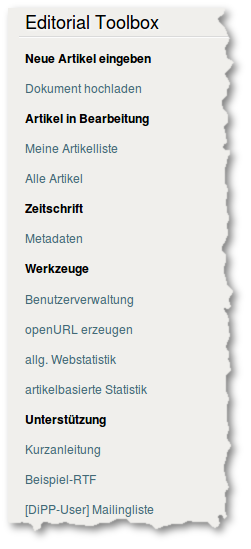
\includegraphics{editorial-toolbox.png}
\caption{Die Editorial Toolbox}\end{figure}


\section{Artikel formatieren}
\label{formatieren::doc}\label{formatieren:artikel-formatieren}\label{formatieren:id1}
Grundlage für eine erfolgreiche Artikelkonvertierung ist die korrekte Verwendung
der \code{Formatvorlage}.
Wichtig sind vor allem die Formate für den  Kopf des Artikels,
der die Metadaten enthält. Anhand der Namen der Absatzformate identifiziert die
Konvertierungsoftware  den Titel, die Autoren, den Abstract, etc. Danach wird eine
Überschrift erster Ordung benötigt, um den eigentliche  Artikeltext von den Metadaten
zu trennen.

\begin{notice}{attention}{Achtung:}
Ein Absatz mit dem Absatzformat ``Überschrift 1'' ist zwingend vorgeschrieben.
Er kann leer sein, muss aber existieren, da der Konverter ansonsten nicht
erkennt, wo der eigentliche Artikel beginnt.
\end{notice}
\begin{figure}[htbp]
\centering
\capstart

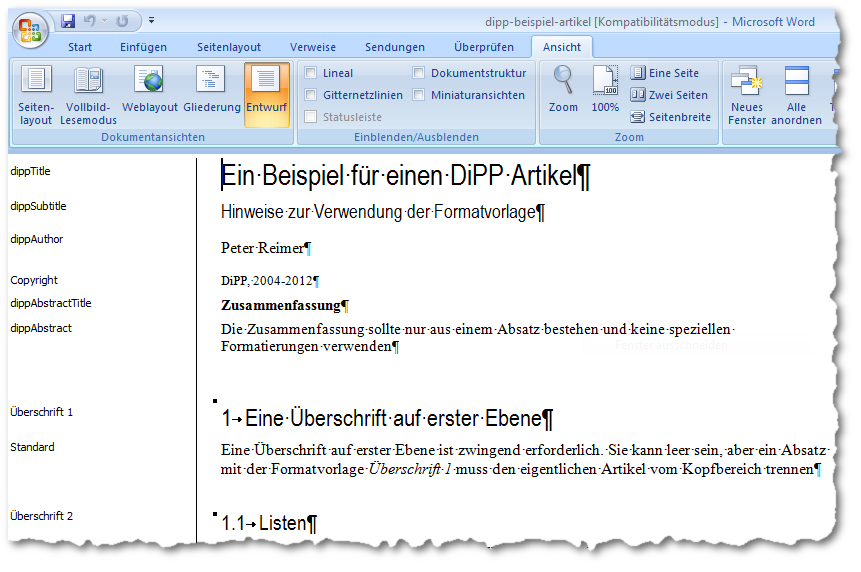
\includegraphics{artikel-in-word.png}
\caption{Ein Artikel mit angewandter Formatvorlage. Entwurfsansicht mit
eingeblendeten Absatzformaten}\end{figure}

Die Standardformatvorlage enthält eine Reihe von Absatzformaten, die im Artikelkopf
angewendet werden können, bzw. müssen. Die bezeichnung und die Reihenfolge ist
wichtig, kann jedoch an die jeweiligen Bedürfnisse angepasst werden. Dafür ist
jedoch auch eine Anpassungen der journalspezifischen XSL und XSLT Datei für die
Konvertierungssoftware notwendig.

\begin{tabulary}{\linewidth}{|L|L|}
\hline
\textbf{
Name der Vorlage
} & \textbf{
Bedeutung
}\\\hline

dippTitle
 & 
Titel der Artikels, erforderlich.
\\\hline

dippSubtitle
 & 
evtl. Untertitel
\\\hline

dippAuthor
 & 
ein oder mehrere Autoren
\\\hline

Copyright
 & 
enthält nach der Konvertierun die URN
\\\hline

dippAbstractTitle
 & 
Überschrift für den Abstract, kann nur einmal vorkommen
\\\hline

dippAbstract
 & 
der Abstract selber
\\\hline
\end{tabulary}


Im Fließtext des Artikel sind die Einschränkungen nicht so restriktiv, es
können auch eigene Formate ergänzt werden, allerdings werden die in Word
gemachten Formatierung wie z.B. Einrückungen, Schriftgrad oder Farbe nicht
automatisch in die HTML Ausgabe übernommen. Diese müssen manuell in den CSS
Dateien nachgezogen werden. Da der Name des Absatzformates zum Klassennamen in
der CSS Datei wird, darf er keine Sonderzeichen oder Leerzeichen enthalten.

In der Regel sollten die Funktionen der Textverarbeitung genutzt werden:
\begin{itemize}
\item {} 
Normale Absätze werden mit der Formatvorlage ``Standard'' formatiert.

\item {} 
Für Überschriften werden die üblichen ``Überschrift 1, Überschrift 2, ...''
verwendet. Aus den Überschriften wird dann das Inhaltsverzeichnis generiert,
das als toc\_html parallel zum Hauptext (fulltext) abeglegt wird. Über ein
entsprechendes Portlet es in einer Randspalte angezeigt werden, siehe {\hyperref[portlets:portlet-toc]{\emph{Inhaltsverzeichnis portlet\_toc}}}.

\item {} 
Fußnoten sollten mit der Fußnotenfunktionen von Word gemacht werden. Zwischen
Fuß- und Endnoten kann wegen fehlender Pagnierung in HTML nicht unterschieden
werden.

\item {} 
Hyperlinks sollten bereits in Word als solche angelegt werden.

\item {} 
Aufzählungen und Nummerierungen sollten mit der entsprechenden Funktion in
Word angelegt werden.

\item {} 
Beschriftungen von Tabellen und Abbildungen sind ebenfalls mit der
entsprechenden Funktion von Word zu erstellen.

\end{itemize}


\subsection{Abbildungen}
\label{formatieren:abbildungen}
Es sind nur pixelbasierte Dateiformat (jpeg, gif, png) möglich, vektorbasierte
Formate wie z.B. wmf oder mit Wordart erstellte Graphiken werden nicht
unterstützt.

Bilder sind in der Auflösung einzubinden, in der sie später im Internet
erscheinen sollen. Abhängig vom Layout der Webseite sollte die Breite 580px
nicht überschreiten. Die Bilder können mit Verweisen (hyperlinks) zu
höherauflösenden Versionen versehen werden, die im Publikationssystem
nachträglich hochgeladen werden können, siehe {\hyperref[zusatzmaterial:zusatzmaterial]{\emph{Zusatzmaterial}}}.


\subsection{Tabellen}
\label{formatieren:tabellen}
Tabellen sollten nicht zu komplex gestaltet werden, d. h. sie sollten nicht
verschachtelt werden und die Größe einzelner Zellen sollten nicht durch Ziehen
der Begrenzungslinie verändert werden. Das Verschmelzen von zwei benachbarten
Zellen ist jedoch möglich. Auch sollte Für die erste Tabellenzeile als Kopfzeile
gesetzt werden. Dazu wird die Zeile in Word markiert und dann über das
Kontektmenü ``Tabelleneigenschaft'', Reiter ``Zeile'' die Option ``Gleiche Kopfzeile
auf jeder Seite wiederholen'' aktiviert. Dadurch wird die Zeile im HTML als header
ausgezeichnet und läßt sich entsprechend über CSS formatieren.
\begin{figure}[htbp]
\centering
\capstart

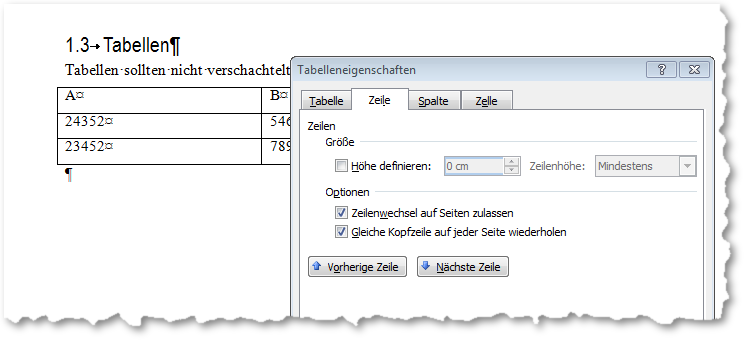
\includegraphics{tabellen-kopf.png}
\caption{Setzen der Eigenschaften für die Kopfzeile der Tabelle}\end{figure}


\section{Zusatzmaterial}
\label{zusatzmaterial:zusatzmaterial}\label{zusatzmaterial::doc}\label{zusatzmaterial:id1}
Unter Zusatzmaterial (supplementary material) lassen sich alle Bestandteile des
Artikel zusammenfassen, die \textbf{nicht} durch die Konvertierung des Artikels aus dem RTF
erhalten werden. Dazu gehören z.B. Bilder in höheren Auflösungen, Multimediale
Inhalte oder der Volltext des Artikel im PDF Format.

Diese Zusatzmaterialien werden über das ``Hinzufügen'' Menu in der grünen
Bearbeitungsleist ergänzt. Zur Verfügung stehen ``Fedora Document'', das für
textbasierte Materialen wie HTML Datein gedacht ist, und ``Fedora Multimedia''
für alle binären Formate: Bilder, PDF Dateien, Film- und Audiodateien, etc.
\begin{figure}[htbp]
\centering
\capstart

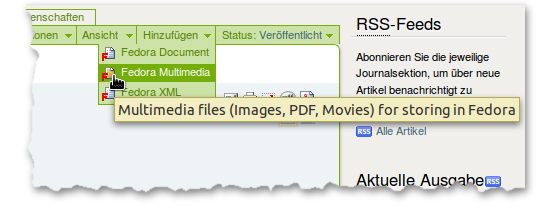
\includegraphics{add_fedoramultimedia.png}
\caption{Hinzufügen von Zusatzmaterial über das ``Hinzufügen'' Menü.}\end{figure}

In dem dann folgendem Formular muss der Titel angegeben werden und die Datei
ausgewählt werden. Das Auswahlfeld ``seperate Listing'' entscheidet darüber, wie
das Zusatzmaterial eingebunden wird:
\begin{description}
\item[{Do not list:}] \leavevmode
Die Datei wird nicht offensichtlich verlinkt, sondern kann beispielsweise
als Bild im HTML Text eingebunden werden. Auf diese Art werden auch Bilder
eingebunden, die durch die Konvertierung aus dem RTF extrahiert werden.

\item[{Alternative Format of the main text:}] \leavevmode
Für die PDF Version des volltextes. Die Datei wird über ein kleines Icon am
rechten oberen Rand verlinkt. Zusätzlich erscheint ein Textlink unterhalb
des Artikel, der zusätzlich eine Größenangabe enthält. Wenn dem Artikel mehrere
PDF Dateien beigefügt werden, wird die im Artikelordner zu oberst stehende Datei
verlinkt

\item[{Supplementary Material:}] \leavevmode
Die Datei wird unterhalb des Artikeltextes in einem separaten Block
angezeigt.

\end{description}
\begin{figure}[htbp]
\centering
\capstart

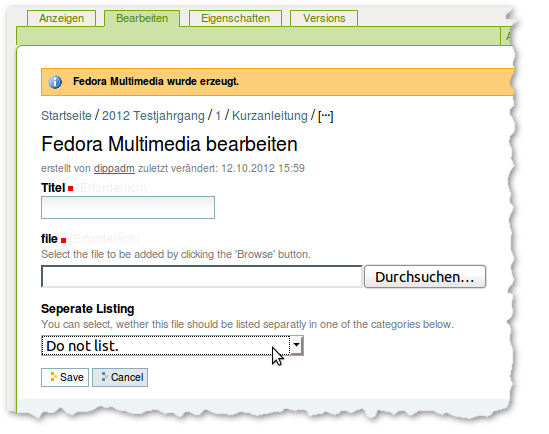
\includegraphics{edit_fedoramultimedia.png}
\caption{Das Bearbeitenformular für Fedora Multimedia Objekte.}\end{figure}

Für einige Multimediadateien werden spezielle Templates angeboten, die über das
``Ansichten'' Menu auswählbar sind. Sie erlauben neben dem standardmäßig
angebotenem Download u.a. das direkte Abspielen von Audiodateien im Browser.
Folgenden Ansichten/Templates stehen zur Auswahl:
\begin{description}
\item[{mp3 view:}] \leavevmode
Abspielen von mp3 Audiodatein mit dem Flowplayer (Flash).

\item[{Simple image view:}] \leavevmode
Einbetten eines Bildes in eine schlichte HTML Seite.

\item[{File view:}] \leavevmode
Nur ein Download Link.

\item[{Flashvideo view:}] \leavevmode
Abspielen von Videodateien im FLV Format mit den Flowplayer (Flash).

\end{description}

Um eine Datei durch eine neue zu ersetzen, sollte sie \textbf{nicht} gelöscht werden
und durch eine neue Datei gleichen Namens ersetzt werden. Sie kann ausgetauscht
werden, in dem man über den ``Bearbeiten'' Reiter wieder die Bearbeitungsmaske
aufruft und unter ``file'' die neue Datei zum Hochladen auswählt. Die übrigen
Einstellungen können bleiben wie sie sind. Beim Speichern wird dann eine neue
Version im Repository abgelegt und die Versionshistorie kann unter dem Reiter
``versions'' eingesehen werden. Diese Historie würde beim Löschen und komplett
neu hochladen verloren gehen.


\section{Kommentare}
\label{kommentare::doc}\label{kommentare:kommentare}
Kommentare zu Artikeln sollen dazu dienen eine Diskussion
zu ermöglichen und sollten daher gewissen wissenschaftlichen Standard genügen.
Zwar durchlaufen die Kommentare keinen Reviewprozess, technischen werden sie
aber genauso behandelt wie der kommentierte Artikel selber, d.h. sie werden
genauso {\hyperref[formatieren:artikel-formatieren]{\emph{formatiert}}} und über die Editorial Toolbox konvertiert.

In der Standardkonfiguration ist die Kommentarfunktion deaktiviert. Um sie
nutzen zu können muss im {\hyperref[glossar:term-zmi]{\emph{ZMI}}} der Wert von
{\hyperref[dipp_properties:allow-persistent-discussion]{\emph{allow\_persistent\_discussion}}} auf ``True'' gesetzt werden.
\begin{figure}[htbp]
\centering
\capstart

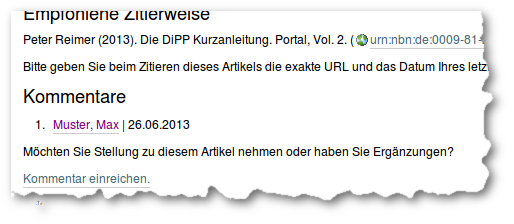
\includegraphics{kommentar-einreichen.png}
\caption{Ein Artikel mit angewandter Formatvorlage. Entwurfsansicht mit
eingeblendeten Absatzformaten}\end{figure}
\begin{figure}[htbp]
\centering
\capstart

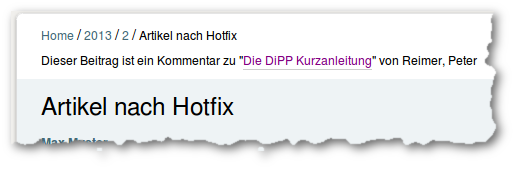
\includegraphics{artikel-ist-kommentar.png}
\caption{Ein Artikel mit angewandter Formatvorlage. Entwurfsansicht mit
eingeblendeten Absatzformaten}\end{figure}


\section{Zählmarken}
\label{metis::doc}\label{metis:zahlmarken}
Damit Texte im Internet von der \href{http://www.vgwort.de/verguetungen/auszahlungen/texte-im-internet.html}{VG Wort} vergütet werden können, müssen die Zugriffe
auf die einzelnen Texte von der Verwertungsgesellschaft erfasst werden.
Zu diesem Zweck müssen die Texte mit sogenannten Zählmarken versehen werden, die man Onlineportal
(\href{https://tom.vgwort.de/portal/index}{T.O.M.}) erhalten kann.


\section{DOAJ}
\label{doaj:t-o-m}\label{doaj::doc}\label{doaj:doaj}
Das


\section{Publikationsworkflow}
\label{workflow:publikationsworkflow}\label{workflow::doc}

\subsection{Upload}
\label{workflow:upload}
Den Einstieg in den Publikationsworkflow erreicht man über die {\hyperref[editorial_toolbox:editorial-toolbox]{\emph{Editorial Toolbox}}}. Der erste Menupunkt unter
Neue Artikel eingeben/ Dokument hochladen führt zu folgender Eingabemaske:
\begin{figure}[htbp]
\centering
\capstart

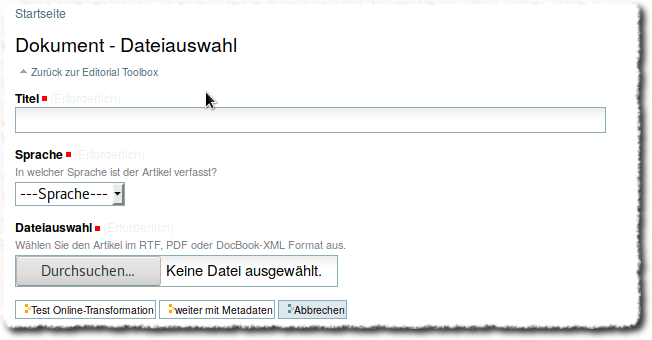
\includegraphics{upload_file_form.png}
\caption{Eingabemaske zum Artikelupload}\end{figure}

Alle drei Felder sind zwingend auszufüllen, bzw. auszuwählen. Da in der Regel mehrere Probleläufe der Konvertierung
nötig sind, bis das ausgegebene HTML den Erwartungen entspricht, hat man an diesem Punkt zwei Wahlmöglichkeiten:

Im ersten Fall \emph{Test Online Transformation} ist keine Angabe von Metadaten notwendig und der eigentliche
Publikationsworkflow wird nicht angestoßen. Der konvertierte Artikel landet in einen Ordner für temporäre Dateien.
Im Fall von \emph{weiter mit Metadaten} muss ein umfangreiches Metadatenformular ausgefüllt werden und der Workflow
wird angestoßen.


\subsection{Worklist}
\label{workflow:worklist}
Je nach Länge und Komplexizität des Artikel dauert die Konvertierung unterschiedlich lange. In beiden Fällen wird man
nach der Konvertierung zur sog. Worklist weitergeleitet.
\begin{figure}[htbp]
\centering
\capstart

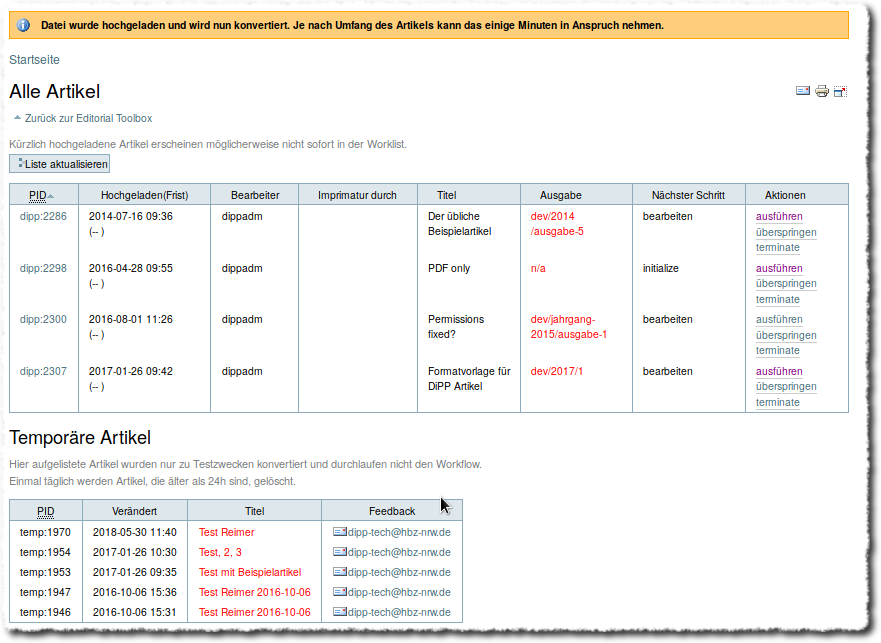
\includegraphics{worklist.png}
\caption{Eine Übersicht aller im Publikationsworkflow befindlichen Artikel. Im unteren
Teil werden die Artikel aufgeführt, die nur zu Testzwecken konvertiert wurden
und nicht veröffentlicht werden sollen.}\end{figure}

Die Worklist ist der Dreh- und Angelpunkt, zu dem man nach jedem einzelnen Schritt
wieder zurückgeleitet wird. Der für den jeweiligen Artikel nächste Schritt ist in der
vorletzten Spalte angegeben, mit dem `ausführen'-Link in der letzten Spalte wird
der Schritt gestartet.


\subsection{1. Schritt: Artikel initialisieren}
\label{workflow:schritt-artikel-initialisieren}
Nach dem Konvertieren befinden sich die Artikel in einem temporären Ordner. Für die
entgültige Veröffentlichng muss zunächst unter `Hierarchische Zuordnung' ein bereits bestehender {\hyperref[ausgaben:volumes-issues]{\emph{Jahrgänge und Ausgaben}}} Ordner
ausgewählt werden. exi
\begin{figure}[htbp]
\centering
\capstart

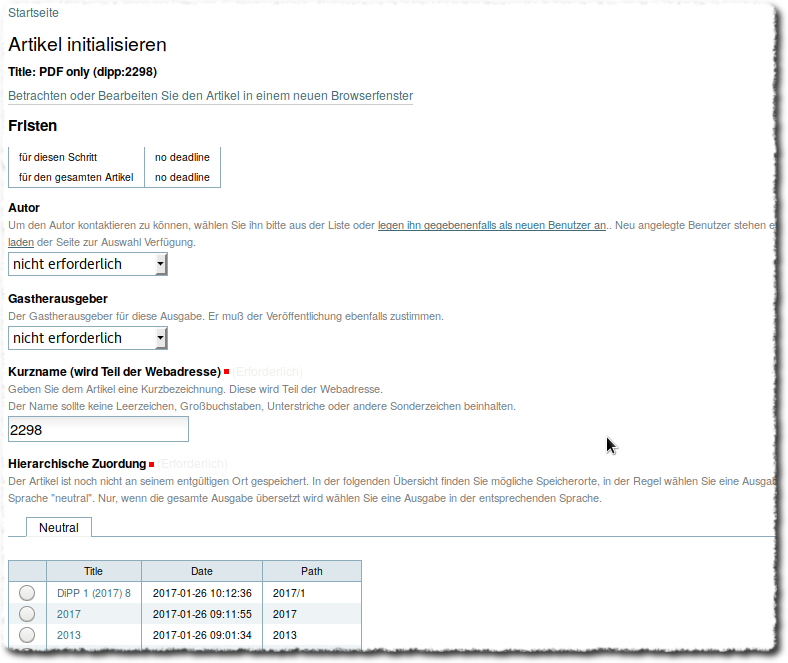
\includegraphics{initialisieren.png}
\caption{Erster Schritt im Workflow: Initialisieren}\end{figure}

Einsortieren der Artikel in eine Ausgabe


\subsection{Artikel bearbeiten}
\label{workflow:artikel-bearbeiten}\begin{figure}[htbp]
\centering
\capstart

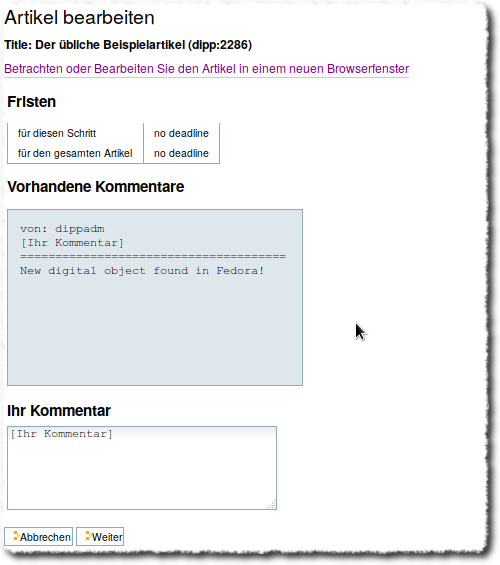
\includegraphics{bearbeiten.png}
\caption{Zweiter Schritt im Workflow: Bearbeiten}\end{figure}


\subsection{Artikel begutachten}
\label{workflow:artikel-begutachten}\begin{figure}[htbp]
\centering
\capstart

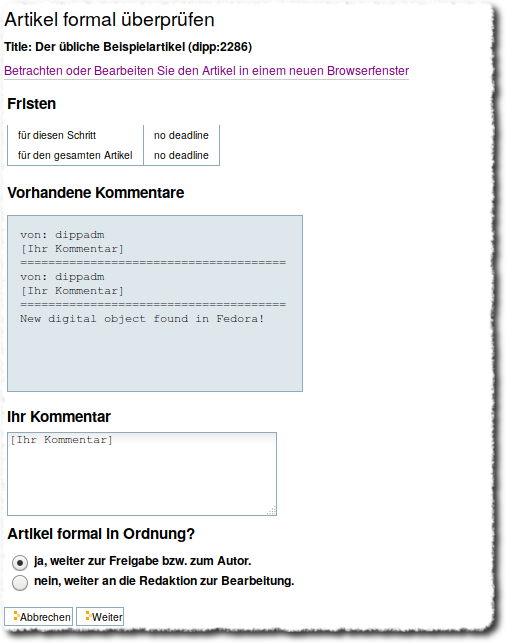
\includegraphics{begutachten.png}
\caption{Dritter Schritt im Workflow: Begutachten}\end{figure}


\subsection{Artikel freischalten}
\label{workflow:artikel-freischalten}\begin{figure}[htbp]
\centering
\capstart

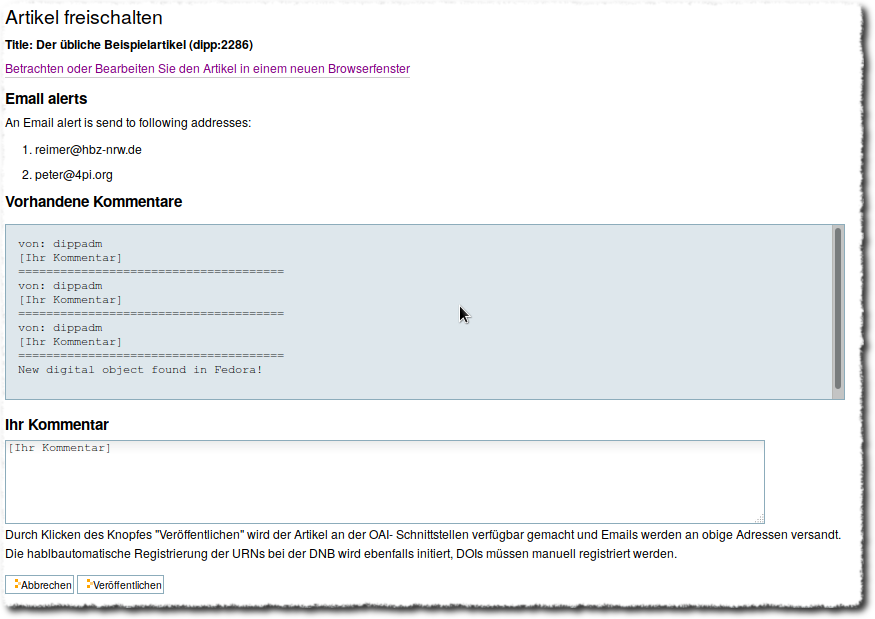
\includegraphics{freischalten.png}
\caption{Letzter Schritt im Workflow: Freischalten}\end{figure}

Bei Veröffentlichung des Artikels wird eine Email an vorher definiert
Adressen {\hyperref[dipp_properties:prop-alertemailaddresses]{\emph{alertEmailAddresses}}} verschickt, der Text ist auch
anpassbar.


\chapter{Jahrgänge und Ausgaben}
\label{ausgaben:jahrgange-und-ausgaben}\label{ausgaben:volumes-issues}\label{ausgaben::doc}
Jahrgänge, Ausgaben und Sonderausgaben dienen dazu, die Artikel hierarchisch
einzuordnen. Im Gegensatz zu Artikeln, die über die Editorial Toolbox
eingestellt werden, werden diese jedoch wie normale Ploneobjekte über das
“Hinzufügen” Menu in der grünen Bearbeitungsleiste angelegt.
\begin{figure}[htbp]
\centering
\capstart

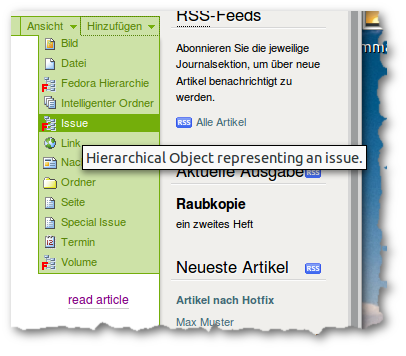
\includegraphics{menu_add_issue.png}
\caption{Hinzufügen von hierarchischen Elementen wie Ausgaben (Issue), Jahrgänge (Volume)
oder Sonderausgaben (Special Issue)}\end{figure}

Sektionen sind keine eigenständigem Objekte, sondern nur eine weiter Eigenschaft
eines Artikels, die über die Metadaten ausgewählt wird.


\section{Jahrgänge, Ausgaben und FedoraHierarchien}
\label{ausgaben:jahrgange-ausgaben-und-fedorahierarchien}\label{ausgaben:volumes}
Diese drei Typen unterscheiden sich prinzipiell nur durch ihre Standardansicht,
die über das ``Ansichten'' Menu ausgewählt werden kann. FedoraHierarchien sollten
nicht mehr verwendet werden und werden nur aus Gründen der
Rückwärtskompatibilität weiterhin vom System unterstützt.

\begin{tabulary}{\linewidth}{|L|L|}
\hline
\textbf{
Typ
} & \textbf{
Ansicht
}\\\hline

Jahrgang (Volume)
 & 
Volume content
\\\hline

Ausgabe (Issue)
 & 
Issue content
\\\hline

FedoraHierarchie
 & 
Base View
\\\hline
\end{tabulary}



\subsection{Volume content}
\label{ausgaben:volume-content}
Diese Template listet nur die direkt im aktuellen Jahrgang angelegten Ausgaben
an. Evtl. weiter vorkommende Jahrgänge, Ausgaben und Fedorahierachien werden
ebenfalls gelistet, alles andere wird ignoriert. Wenn die untergeordneten
Ausgaben Titelbilder haben, können diese eingeblendet werden, siehe
{\hyperref[dipp_properties:prop-volume-show-covers]{\emph{volume\_show\_covers}}}


\subsection{Issue content}
\label{ausgaben:issue-content}

\section{Sonderausgaben}
\label{ausgaben:id1}\label{ausgaben:sonderausgaben}

\section{Sektionen}
\label{ausgaben:sektionen}\label{ausgaben:id2}

\chapter{Portlets}
\label{portlets::doc}\label{portlets:portlets}

\section{Suche \texttt{portlet\_articlesearch}}
\label{portlets:portlet-articlesearch}\label{portlets:suche-portlet-articlesearch}
Stellt einen Suchschlitz zur Verfügung, der als Ergebnis nur Artikel zurückgibt (FedoraArticle),
keine normalen Webseiten.


\section{Automatisches Inhaltsverzeichnis \texttt{portlet\_autotoc}}
\label{portlets:automatisches-inhaltsverzeichnis-portlet-autotoc}\label{portlets:portlet-autotoc}
Bindet das mit jeder Versionierung des Artikels aktualisierte Inhaltsverzeichnis
ein. Zur Konfiguration siehe {\hyperref[dipp_properties:prop-deepest-toc-level]{\emph{deepest\_toc\_level}}}


\section{Aktuelle Ausgabe \texttt{portlet\_currentissue}}
\label{portlets:portlet-currentissue}\label{portlets:aktuelle-ausgabe-portlet-currentissue}
Eine Auflistung der Artikel der aktuellen Ausgabe. Wenn der Ausgabe ein Titelbild
beigefügt wurde, wird dieses verkleinert dargestellt. Auch eine Sortierung nach
Sektionen wird vorgenommen. Weitere Konfiguration ist durch folgende Properties
möglich: {\hyperref[dipp_properties:prop-articles-in-portlet]{\emph{articles\_in\_portlet}}}, {\hyperref[dipp_properties:prop-authors-in-portlet]{\emph{authors\_in\_portlet}}}.


\section{DiPP Navigation \texttt{portlet\_dippnav}}
\label{portlets:dipp-navigation-portlet-dippnav}\label{portlets:portlet-dippnav}
Kleine Navigation mit Links zur ``Editoral Toolbox'', dem Plone Setup und dem
sog. ``Website Manager'', der nicht anderes ist als die Inhaltsansicht der
obersten Verzeichnisebene.


\section{Editorial Toolbox \texttt{portlet\_editorialtoolbox}}
\label{portlets:portlet-editorialtoolbox}\label{portlets:editorial-toolbox-portlet-editorialtoolbox}
Siehe eigene Seite: {\hyperref[editorial_toolbox:editorial-toolbox]{\emph{Editorial Toolbox}}}.


\section{Feeds \texttt{portlet\_feeds}}
\label{portlets:portlet-feeds}\label{portlets:feeds-portlet-feeds}
Dieses Portlet enthält eine Liste der verfügbaren {\hyperref[glossar:term-rss]{\emph{RSS}}}-Feeds. Ein Feed
mit allen veröffentlichen Artikeln steht immer zur Verfügung, wenn die Artikel
noch in einzelne Sektionen eingeordnet werden, stehen auch seperate Feeds hierfür
zum abonnieren bereit.


\section{ISSN \texttt{portlet\_issn}}
\label{portlets:issn-portlet-issn}\label{portlets:portlet-issn}
Ein Portlet, das einfach  nur die ISSN-Nummer wiedergibt. Sie muss in
den dipp\_properties angegeben werden, siehe {\hyperref[metadata_properties:prop-issn]{\emph{issn}}}.


\section{Newsletter \texttt{portlet\_newsletter}}
\label{portlets:portlet-newsletter}\label{portlets:newsletter-portlet-newsletter}
Ein Portlet, das eine Anmeldemaske für einen Newsletter anbietet. Erfordert die
Installation und Konfiguration des PloneGazette Produktes.


\section{Aktuelle Artikel \texttt{portlet\_recentarticles}}
\label{portlets:aktuelle-artikel-portlet-recentarticles}\label{portlets:portlet-recentarticles}
Chronologische Aufzählung der letzten fünf Artikel, Sektionen und
{\hyperref[dipp_properties:prop-authors-in-portlet]{\emph{authors\_in\_portlet}}} werden ausgewertet.


\section{Suche \texttt{portlet\_search}}
\label{portlets:suche-portlet-search}\label{portlets:portlet-search}
Alternative Positionierung der Suchmaske.


\section{Inhaltsverzeichnis \texttt{portlet\_toc}}
\label{portlets:inhaltsverzeichnis-portlet-toc}\label{portlets:portlet-toc}
Stellt das das generierte Inhaltsverzeichnis \emph{toc\_html} dar.
Das Inhaltsverzeichnis wird bei der Konvertierung einmalig automatisch generiert
und nicht aktualisiert, wenn z.B. ein Tippfehler im HTML korrigiert wird.
Wird nur bei Artikeln eingeblendet. Die Alternative {\hyperref[portlets:portlet-autotoc]{\emph{Automatisches Inhaltsverzeichnis portlet\_autotoc}}} hingegen wird bei
jeder Versionierung des Artikeltextes ebenfall aktualisiert.


\chapter{Konfiguration}
\label{konfiguration:konfiguration}\label{konfiguration::doc}
Die meisten Einstellungen werden in sogenannten Plone Property Sheets gespeichert.
Diese findet man unter \emph{ZMI \(\rightarrow\) portal\_properties}.
Neben dem Standardsheet site\_properties gibt es noch vier eigene Sheets, relevant sind
für das Publikationssystem:


\section{dipp\_properties (DiPP properties)}
\label{dipp_properties:dipp-properties-dipp-properties}\label{dipp_properties::doc}
enthält Konfigurationen, die das Erscheinungsbild von Ausgaben und
Artikeln beeinflussen.


\subsection{ISSN}
\label{dipp_properties:prop-issn}\label{dipp_properties:issn}
Die \emph{International Standard Serial Number}. Kann mit erscheinen der ersten Artikel
bei der Deutschen Nationalbibliothek beantragt werden.


\subsection{alertEmailAddresses}
\label{dipp_properties:prop-alertemailaddresses}\label{dipp_properties:alertemailaddresses}
Eine Liste mit E-Mail Adressen, die bei Veröffentlichung eines Artikel
benachrichtigt werden.

Default:

\begin{Verbatim}[commandchars=\\\{\}]
dipp@hbz-nrw.de
\end{Verbatim}


\subsection{alertEmailText}
\label{dipp_properties:prop-alertemailtext}\label{dipp_properties:alertemailtext}
Text dieser Email:

\begin{Verbatim}[commandchars=\\\{\}]
Das Journal "\%(journal)s" hat einen neuen Artikel veröffentlicht:
\%(citation)s

URL: \%(url)s
DataCite XML: \%(url)s/metadata/datacite
\end{Verbatim}

Zur Verfügung stehende Platzhalter:

\begin{tabulary}{\linewidth}{|L|L|}
\hline
\textbf{
Name
} & \textbf{
Bedeutung
}\\\hline

journal
 & 
Name des journals
\\\hline

url
 & 
URL des Artikels
\\\hline

citation
 & 
Bibliographischen Zitat des Artikels
\\\hline
\end{tabulary}



\subsection{citation\_format}
\label{dipp_properties:citation-format}
String, der zum Formatieren der empfolenen Zitierweise verwendet wird, wie sie
unter dem Artikel bzw. auf der Seite mit den Metadaten zu dinen ist.

Default:

\begin{Verbatim}[commandchars=\\\{\}]
\%(authors)s (\%(year)s). \%(title)s. \%(journal)s, Vol. \%(volume)s. (\%(urn)s)
\end{Verbatim}

Zur Verfügung stehende Platzhalter:

\begin{tabulary}{\linewidth}{|L|L|}
\hline
\textbf{
Name
} & \textbf{
Bedeutung
}\\\hline

authors
 & 
Liste der Autoren, kann durch weitere Parameter detailierter
formatiert werden
\\\hline

title
 & 
Titel des Artikels
\\\hline

journal
 & 
Name des Journals
\\\hline

volume
 & 
Jahrgang
\\\hline

issue
 & 
Ausgabe
\\\hline

startpage
 & 
erste Seite (bei PDF)
\\\hline

endpage
 & 
letzte Seite (bei PDF)
\\\hline

year
 & 
Jahreszahl, wird aus den Datum der Veröffentlich extrahiert
\\\hline

date
 & 
Datum der Veröffentlichung
\\\hline

id
 & 
die PID ohne des Prefix `dipp:'
\\\hline

urn
 & 
Der URN
\\\hline
\end{tabulary}



\subsection{short\_citation\_format}
\label{dipp_properties:short-citation-format}\label{dipp_properties:prop-short-citation-format}
String, der zum Formatieren der verkürzten Zitierweise verwendet wird. Wird aus
den Metadaten erzeugt, die auch im Plone Katalog indexiert sind und keinen
Aufruf von Fedora erfordern. Kann z.B. auf den Inhaltsverzeichnissen oder den
Feeds verwendet werden.

Default:

\begin{Verbatim}[commandchars=\\\{\}]
\%(journal)s, Vol. \%(volume)s, Iss. \%(issue)s
\end{Verbatim}

Zur Verfügung stehende Platzhalter:

\begin{tabulary}{\linewidth}{|L|L|}
\hline
\textbf{
Name
} & \textbf{
Bedeutung
}\\\hline

journal
 & 
Name des Journals
\\\hline

journal\_shortname
 & 
Abkürzung des Journals, siehe {\hyperref[metadata_properties:prop-journalname-abbr]{\emph{journalname\_abbr}}}
\\\hline

volume
 & 
Jahrgang
\\\hline

issue
 & 
Ausgabe
\\\hline

startpage
 & 
erste Seite (bei PDF)
\\\hline

endpage
 & 
letzte Seite (bei PDF)
\\\hline

year
 & 
Jahreszahl, wird aus den Datum der Veröffentlich extrahiert
\\\hline

issuedate
 & 
Datum der Veröffentlichung
\\\hline

urn
 & 
Der URN
\\\hline
\end{tabulary}



\subsection{issue\_date\_format}
\label{dipp_properties:prop-issue-date-format}\label{dipp_properties:issue-date-format}
Formatierung des Ausgabendatums in Listen aller Ausgaben. \href{http://docs.python.org/2/library/datetime.html\#strftime-and-strptime-behavior}{http://docs.python.org/2/library/datetime.html\#strftime-and-strptime-behavior}

Default:

\begin{Verbatim}[commandchars=\\\{\}]
\%b \%Y
\end{Verbatim}


\subsection{hide\_current\_issue}
\label{dipp_properties:hide-current-issue}\label{dipp_properties:id1}
Bestimmt, ob die aktuelle Ausgabe im all\_issues Template angezeigt werden soll. Bei Verwendung eines currentissue
Links kann das evtl. sinnvoll sein.

Default:

\begin{Verbatim}[commandchars=\\\{\}]
\PYG{n+nb+bp}{False}
\end{Verbatim}


\subsection{show\_recommended\_citation}
\label{dipp_properties:show-recommended-citation}
Soll unterhalb des Artikels das bibliographische Zitat angezeigt werden?

Default:

\begin{Verbatim}[commandchars=\\\{\}]
\PYG{n+nb+bp}{True}
\end{Verbatim}


\subsection{show\_classified\_subjects}
\label{dipp_properties:show-classified-subjects}
Sollen im Artikelkopf die normierten Schlagworte angezeigt werden?

Default:

\begin{Verbatim}[commandchars=\\\{\}]
\PYG{n+nb+bp}{False}
\end{Verbatim}


\subsection{show\_review\_history}
\label{dipp_properties:show-review-history}
Sollen im Artikelkopf die Daten für Einreichung und Annahme angezeigt werden?

Default:

\begin{Verbatim}[commandchars=\\\{\}]
\PYG{n+nb+bp}{False}
\end{Verbatim}


\subsection{initials\_only}
\label{dipp_properties:initials-only}
Im bibliographischen Zitat: Sollen bei den Autoren nur die Initialen angezeigt
werden statt des ausgeschriebenen Vornamens:

Default:

\begin{Verbatim}[commandchars=\\\{\}]
\PYG{n+nb+bp}{False}
\end{Verbatim}


\subsection{firstnamefirst}
\label{dipp_properties:firstnamefirst}
Im bibliographischen Zitat: Sollen erst die Vornamen angezeigt werden?

Default:

\begin{Verbatim}[commandchars=\\\{\}]
\PYG{n+nb+bp}{False}
\end{Verbatim}


\subsection{initials\_period}
\label{dipp_properties:initials-period}
Im bibl. Zitat: Sollen ein Punkt hinter die Initialen?

Default:

\begin{Verbatim}[commandchars=\\\{\}]
\PYG{n+nb+bp}{False}
\end{Verbatim}


\subsection{comma\_separated}
\label{dipp_properties:comma-separated}
Im bibl. Zitat: wenn der Vorname nach dem Nachnamen kommt (firstnamefirst =
false), sollen sie durch ein Komma getrennt werden:

Default:

\begin{Verbatim}[commandchars=\\\{\}]
\PYG{n+nb+bp}{False}
\end{Verbatim}


\subsection{last\_author\_suffix}
\label{dipp_properties:last-author-suffix}
Im  bibl. Zitat: wenn der letzte Autor z.B. durch ein `und' abgetrennt werden
soll.

Default:

\begin{Verbatim}[commandchars=\\\{\}]
\textless{}leer\textgreater{}
\end{Verbatim}


\subsection{articles\_in\_portlet}
\label{dipp_properties:prop-articles-in-portlet}\label{dipp_properties:articles-in-portlet}
Im Portlet ``Current Issue'': Sollen die Artikel aufgelistet werden? Sonst
escheint nur ein Link auf die Ausgabe, evtl. mit Bild.

Default:

\begin{Verbatim}[commandchars=\\\{\}]
\PYG{n+nb+bp}{True}
\end{Verbatim}


\subsection{authors\_in\_portlet}
\label{dipp_properties:prop-authors-in-portlet}\label{dipp_properties:authors-in-portlet}
Im Portlet ``Current Issue'': Sollen auch die Autoren gelistet werden?

Default:

\begin{Verbatim}[commandchars=\\\{\}]
\PYG{n+nb+bp}{True}
\end{Verbatim}


\subsection{allow\_persistent\_discussion}
\label{dipp_properties:id2}\label{dipp_properties:allow-persistent-discussion}
Wenn True, wird unterhalb eines Artikels eine Liste mit Kommentaren und ein Link
zum Einreichen eines eigenen Kommentares eingeblendet. Kommentare sind
ihrerseits wieder begutachtete Artikel.

Default:

\begin{Verbatim}[commandchars=\\\{\}]
\PYG{n+nb+bp}{False}
\end{Verbatim}


\subsection{volume\_show\_covers}
\label{dipp_properties:prop-volume-show-covers}\label{dipp_properties:volume-show-covers}
Wenn True, werden auf der Inhaltsseite der Jahrgänge die Titelseiten der
Ausgaben angezeigt, soweit vorhanden.

Default:

\begin{Verbatim}[commandchars=\\\{\}]
\PYG{n+nb+bp}{False}
\end{Verbatim}


\subsection{issue\_show\_abstracts}
\label{dipp_properties:issue-show-abstracts}
Wenn True, werden auf der Inhaltsseite der Ausgaben die verfügbaren Abstracts
der Artikel verlinkt.

Default:

\begin{Verbatim}[commandchars=\\\{\}]
\PYG{n+nb+bp}{False}
\end{Verbatim}


\subsection{issue\_show\_full\_abstracts}
\label{dipp_properties:issue-show-full-abstracts}
Wenn True, werden auf der Inhaltsseite der Ausgaben die Abstracts in voller
Länge angezeigt.

Default:

\begin{Verbatim}[commandchars=\\\{\}]
\PYG{n+nb+bp}{False}
\end{Verbatim}


\subsection{issue\_show\_pdf\_link}
\label{dipp_properties:issue-show-pdf-link}
Wenn True, werden auf der Inhaltsseite der Ausgaben vorhandene PDFs direkt
verlinkt.

Default:

\begin{Verbatim}[commandchars=\\\{\}]
\PYG{n+nb+bp}{False}
\end{Verbatim}


\subsection{issue\_show\_short\_citation}
\label{dipp_properties:issue-show-short-citation}
Wenn True, werden auf der Inhaltsseite der Ausgaben zu den Artikeln das
bibligraphische Zitat in Kurzform angezeigt, siehe
{\hyperref[dipp_properties:prop-short-citation-format]{\emph{short\_citation\_format}}}

Default:

\begin{Verbatim}[commandchars=\\\{\}]
\PYG{n+nb+bp}{False}
\end{Verbatim}


\subsection{issue\_sort\_on}
\label{dipp_properties:issue-sort-on}
Bestimmt auf der Inhaltsseite der Ausgaben, wonach die Artikelliste sortiert
werden soll. Möglich sind alle sortierbaren Attribute der Artikel, z.B.
getIssue, getIssueDate, getVolume, getObjPositionInParent. Letzteres ermöglicht
eine manuelle Sortierung, die Reihenfolge im Elternorder (Ausgabe) übernommen
wird.

Default:

\begin{Verbatim}[commandchars=\\\{\}]
\PYG{n}{getObjPositionInParent}
\end{Verbatim}


\subsection{issue\_sort\_order}
\label{dipp_properties:issue-sort-order}
Aufsteigende (ascending) oder absteigende (reverse) Sortierung der Artikel

Default:

\begin{Verbatim}[commandchars=\\\{\}]
\PYG{n}{ascending}
\end{Verbatim}


\subsection{discussion\_time}
\label{dipp_properties:discussion-time}
(wird nicht verwendet)


\subsection{fedora\_time\_format}
\label{dipp_properties:fedora-time-format}
String um die Fedorazeitstempel im ZMI lesbarer anzuzeigen. Sollte eigentlich
niemals geändert werden müssen.

Default:

\begin{Verbatim}[commandchars=\\\{\}]
\%Y-\%m-\%dT\%H:\%M:\%SZ
\end{Verbatim}


\subsection{issue\_date\_format}
\label{dipp_properties:id3}
Wenn nicht leer, wird das Datum auf der Ausgabenseite mit dem hier angegebenen
String formatiert. Wenn leer, wird auch kein Datum angezeigt.

Default:

\begin{Verbatim}[commandchars=\\\{\}]
\textless{}leer\textgreater{}
\end{Verbatim}


\subsection{recent\_articles\_range}
\label{dipp_properties:prop-recent-articles-range}\label{dipp_properties:recent-articles-range}
Alter (in Tagen) des ältesten Artikels der durch das recent\_article Template
angezeigt werden soll.

Default:

\begin{Verbatim}[commandchars=\\\{\}]
\PYG{l+m+mi}{30}
\end{Verbatim}


\subsection{deepest\_toc\_level}
\label{dipp_properties:prop-deepest-toc-level}\label{dipp_properties:deepest-toc-level}
Die niedrigste Überschriftenebene, die im  {\hyperref[portlets:portlet-autotoc]{\emph{Automatisches Inhaltsverzeichnis portlet\_autotoc}}} Inhaltsverzeichnis (TOC) des Artikels noch
angezeigt werden soll. Es ist zu beachten, dass die erste Ebene h2 ist. Um die
ersten drei Ebenen anzuzegen, muss der Wert auf 4 gesetzt werden. Der globale Wert
kann auf für einen einelnen Artikel überschrieben werden, wenn im ZMI eine entsprechend
benannte Property angelegt wird. Das TOC wird aktualisiert, wenn vom Artikel eine neue
Version angelegt wird.

Default:

\begin{Verbatim}[commandchars=\\\{\}]
\PYG{l+m+mi}{6}
\end{Verbatim}


\subsection{awstats\_id}
\label{dipp_properties:prop-awstats-id}\label{dipp_properties:awstats-id}
Wenn der Name der AWStats Konfgurationsdatei ``awstats.ejournal.conf'' lautet, ist die
awstats\_id ``ejournal'' Daraus ergeben sich dann die geparsten Logfiles zu z.B
``awstats112011.ejournal.txt'' Daraus werden dann die Zugriffstatiskten einzelner Artikel
bzw. Artikeldateien generiert.

Default:

\begin{Verbatim}[commandchars=\\\{\}]
\textless{}leer\textgreater{}
\end{Verbatim}


\subsection{enable\_ebookey}
\label{dipp_properties:id4}\label{dipp_properties:enable-ebookey}
Zeige unter Volltext einen Link zur per ebookey erzeugten epub-Version des Artikeln.

Default:

\begin{Verbatim}[commandchars=\\\{\}]
\PYG{n+nb+bp}{False}
\end{Verbatim}


\subsection{orcid\_cli}
\label{dipp_properties:orcid-cli}\label{dipp_properties:id5}

\subsection{twitter\_username}
\label{dipp_properties:id6}\label{dipp_properties:twitter-username}
Benutzername bei twitter, ohne führendes @:

Default:

\begin{Verbatim}[commandchars=\\\{\}]
\textless{}leer\textgreater{}
\end{Verbatim}


\subsection{sharing\_image}
\label{dipp_properties:id7}\label{dipp_properties:sharing-image}

\section{metadata\_properties (QDC Metadata properties)}
\label{metadata_properties:metadata-properties-qdc-metadata-properties}\label{metadata_properties::doc}
einige Standardwerte für die Qualifizierten Dublin Core Metadaten.


\subsection{journalname}
\label{metadata_properties:prop-journalname}\label{metadata_properties:journalname}

\subsection{journalname\_abbr}
\label{metadata_properties:journalname-abbr}\label{metadata_properties:prop-journalname-abbr}
Kurzform des Journalnamens. Kann zum Beispiel in der kurzen Version der Zitierweise
angewendet werden, z.B. JOE statt Journal of Examples.

Default:

\begin{Verbatim}[commandchars=\\\{\}]
\textless{}leer\textgreater{}
\end{Verbatim}


\subsection{publisher}
\label{metadata_properties:publisher}\label{metadata_properties:prop-publisher}

\subsection{issn}
\label{metadata_properties:prop-issn}\label{metadata_properties:issn}

\subsection{doi\_prefix}
\label{metadata_properties:prop-doi-prefix}\label{metadata_properties:doi-prefix}
Prefix für alle vergebenen DOI. DOIs bestehen aus einem internen Suffix und
einem von einem Provider wie CrossRef oder der TIB vergebenen Prefix, das
üblicherweise die Form \emph{10.xxxx} hat. \emph{10.5072} ist ein spezieller Testprefix.

Ohne Angabe des Prefix steht das entsprechende Feld im Metadatenformular nicht
zur Verfügung.

Default:

\begin{Verbatim}[commandchars=\\\{\}]
\textless{}leer\textgreater{}
\end{Verbatim}


\subsection{default\_pubType}
\label{metadata_properties:default-pubtype}\label{metadata_properties:prop-default-pubtype}
Default:

\begin{Verbatim}[commandchars=\\\{\}]
\PYG{n}{article}
\end{Verbatim}


\subsection{default\_docType}
\label{metadata_properties:prop-default-doctype}\label{metadata_properties:default-doctype}
Default:

\begin{Verbatim}[commandchars=\\\{\}]
\PYG{n}{text}
\end{Verbatim}


\subsection{default\_language}
\label{metadata_properties:default-language}\label{metadata_properties:prop-default-language}

\subsection{available\_languages}
\label{metadata_properties:available-languages}\label{metadata_properties:prop-available-languages}
Default:

\begin{Verbatim}[commandchars=\\\{\}]
\PYG{n}{ger}
\PYG{n}{eng}
\PYG{n}{fra}
\PYG{n}{ita}
\PYG{n}{spa}
\end{Verbatim}


\section{member\_properties (Extended member properties)}
\label{member_properties:member-properties-extended-member-properties}\label{member_properties::doc}
enthält Konfigurationen für das Anmeldeformular, d.h. welche Daten sind
erforderlich bzw. sollen überhaupt angezeigt werde.
\begin{itemize}
\item {} 
academictitle\_visible

\item {} 
academictitle\_required

\item {} 
givenname\_visible

\item {} 
givenname\_required

\item {} 
surname\_visible

\item {} 
surname\_required

\item {} 
organization\_visible

\item {} 
organization\_required

\item {} 
postaladdress\_visible

\item {} 
postaladdress\_required

\item {} 
postalcode\_visible

\item {} 
postalcode\_required

\item {} 
phone\_visible

\item {} 
phone\_required

\item {} 
location\_visible

\item {} 
location\_required

\item {} 
areas\_of\_expertise

\item {} 
mail\_password\_visible

\end{itemize}


\section{dippreview\_properties (DiPPReview properties)}
\label{dippreview_properties:dippreview-properties-dippreview-properties}\label{dippreview_properties::doc}
Enthält Konfigurationen für den Peer Review (Fristen, Anzahl Gutachter,
...)


\section{site\_properties}
\label{site_properties:site-properties}\label{site_properties::doc}
Hierbeit handelt es sich um Plones Standard Propertysheet, in dem auch die allgemeiner Konfiguration
gespeichert wird. Da die Konfiguration des Trackings nicht Dipp spezifisch ist, wurde sie ebenfalls
hier hinterlegt.


\subsection{analytics\_id}
\label{site_properties:analytics-id}\label{site_properties:id1}
Matomo ID der Website. Kann dem Tracking-Code in den Matomoeinstellungen entnommen werden.
Obwohl die ID immer ein ganzzahliger Wert ist, wird er hier als String hinterlegt

Default:

\begin{Verbatim}[commandchars=\\\{\}]
\textless{}leer\textgreater{}
\end{Verbatim}


\subsection{analytics\_server}
\label{site_properties:id2}\label{site_properties:analytics-server}
URL des Servers, auf dem die Matomoinstallation läuft. Im DiPP Zusammenhang wird das
aktuell alkyoneus.hbz-nrw.de/piwik oder porphyrion.hbz-nrw.de/piwik sein

Default:

\begin{Verbatim}[commandchars=\\\{\}]
\textless{}leer\textgreater{}
\end{Verbatim}


\subsection{analytics\_javascript}
\label{site_properties:analytics-javascript}\label{site_properties:id3}
JavaScript-Tracking-Code für Matomo wird in jeder Seite über das webstats Makro eingebunden.
Das gleichnamige Pagetemplate enthält auch die javascriptfreie Trackingvariante über ein Bild.
Die Variablen \%s werden durch {\hyperref[site_properties:analytics-id]{\emph{analytics\_id}}} bzw {\hyperref[site_properties:analytics-server]{\emph{analytics\_server}}} ersetzt.

Default:

\begin{Verbatim}[commandchars=\\\{\}]
var \_paq = \_paq \textbar{}\textbar{} [];
/* tracker methods like "setCustomDimension" should be called before "trackPageView" */
\_paq.push(['trackPageView']);
\_paq.push(['enableLinkTracking']);
(function() \PYGZob{}
    var u="//\%s/";
    \_paq.push(['setTrackerUrl', u+'piwik.php']);
    \_paq.push(['setSiteId', '\%s']);
    var d=document, g=d.createElement('script'), s=d.getElementsByTagName('script')[0];
    g.type='text/javascript'; g.async=true; g.defer=true; g.src=u+'piwik.js'; s.parentNode.insertBefore(g,s);
\PYGZcb{})();
\end{Verbatim}


\subsection{analytics\_javascript\_notfound}
\label{site_properties:analytics-javascript-notfound}\label{site_properties:id4}
JavaScript-Tracking-Code für Matomo wird in jeder Seite über das webstats Makro eingebunden.
Die Variablen \%s werden durch {\hyperref[site_properties:analytics-id]{\emph{analytics\_id}}} bzw {\hyperref[site_properties:analytics-server]{\emph{analytics\_server}}} ersetzt.
Dies ist ein \href{https://matomo.org/faq/how-to/faq\_60/}{spezieller Trackingcode}, der nur für 404 Seiten verwendet wird.

Default:

\begin{Verbatim}[commandchars=\\\{\}]
var \_paq = \_paq \textbar{}\textbar{} [];
/* tracker methods like "setCustomDimension" should be called before "trackPageView" */
\_paq.push(['setDocumentTitle',  '404/URL = ' +  encodeURIComponent(document.location.pathname+document.location.search) + '/From = ' + encodeURIComponent(document.referrer)]);
\_paq.push(['trackPageView']);
\_paq.push(['enableLinkTracking']);
(function() \PYGZob{}
    var u="//\%s/";
    \_paq.push(['setTrackerUrl', u+'piwik.php']);
    \_paq.push(['setSiteId', '\%s']);
    var d=document, g=d.createElement('script'), s=d.getElementsByTagName('script')[0];
    g.type='text/javascript'; g.async=true; g.defer=true; g.src=u+'piwik.js'; s.parentNode.insertBefore(g,s);
\PYGZcb{})();
\end{Verbatim}


\chapter{Changelog}
\label{changelog::doc}\label{changelog:changelog}

\section{DiPP 2.26 (2019-??-??)}
\label{changelog:dipp-2-26-2019}\begin{itemize}
\item {} 
Support for CC Licences added

\item {} 
improved email alert with bibl. citation and direct
link to datacit xml

\end{itemize}


\section{DiPP 2.25.1 (2018-01-19)}
\label{changelog:dipp-2-25-1-2018-01-19}\begin{itemize}
\item {} 
minor bugfix

\end{itemize}


\section{DiPP 2.25 (2018-01-19)}
\label{changelog:dipp-2-25-2018-01-19}\begin{itemize}
\item {} 
Piwik/Matomo
\begin{itemize}
\item {} 
Special Piwik/Matomo code also for \href{https://matomo.org/faq/how-to/faq\_60/}{404 Pages} including referrer

\item {} 
multipingual Privacypage with Piwik opt-out

\item {} 
Tracking JS Code included via macro and propertysheet, no need to
customize the maintemplate any more

\end{itemize}

\item {} 
Bugfixes, code cleanup, \href{https://www.python.org/dev/peps/pep-0008/}{PEP 8}

\item {} 
ZMI improvements on manage pages of Fedoraobjects, i.e. view tab
for folderish types.

\item {} 
Paragraph numbers added to Wordtemplate and CSS

\end{itemize}


\section{DiPP 2.24 (unreleased)}
\label{changelog:dipp-2-24-unreleased}\label{changelog:pep-8}\begin{itemize}
\item {} 
use https for DOI resolving according to display guidelines of
\href{https://support.datacite.org/v1.0/docs/datacite-doi-display-guidelines}{DataCite} and \href{https://www.crossref.org/display-guidelines/}{Crossref}

\item {} 
DataCite Metadata Schema 4.0

\item {} 
Support for TwitterCard and Opengraph Metatags.

\item {} 
Updated Documentation

\end{itemize}


\section{DiPP 2.23 (2016-10-07)}
\label{changelog:dipp-2-23-2016-10-07}\label{changelog:crossref}\begin{itemize}
\item {} 
fixed initialisation problem for contenttypes

\end{itemize}


\section{DiPP 2.22 (2016-07-27)}
\label{changelog:dipp-2-22-2016-07-27}\begin{itemize}
\item {} 
fixed problem when installing permissions

\end{itemize}


\section{DiPP 2.21 (2016-07-27)}
\label{changelog:dipp-2-21-2016-07-27}\begin{itemize}
\item {} 
improved print stylesheet

\item {} 
ebookey can be enabled in dipp\_properties, since it only works for journals
with html versions of the articles. Note: cover image required, but without
alpha channel

\item {} 
persistent urls for metadata

\end{itemize}


\section{DiPP 2.20 (unreleased)}
\label{changelog:dipp-2-20-unreleased}\begin{itemize}
\item {} 
show access statistics from AWStats directly in Plone, proteced by
dedicated permission setting

\item {} 
fixed reCAPTCHA. Validation expected two words, which failed for single
(house)numbers

\item {} 
new portlet with automatic generated table of contents portlet\_autotoc
(requires dipp.tools version 0.6)

\item {} 
ebook support

\end{itemize}


\section{DiPP 2.19 (2014-08-29)}
\label{changelog:dipp-2-19-2014-08-29}\begin{itemize}
\item {} 
javascript support for metadata form. adding new fields does not require
reload of entire form

\item {} 
new get\_location method, which passes the url of a ploneobject to fedora
based on IP and port and bypassing the VHM.

\item {} 
fixed permission problem in issue\_portlet

\item {} 
orcid fix for https connections

\item {} 
improved DOI handling

\item {} 
show pdf/a next to pdf

\end{itemize}


\section{DiPP 2.18 (2014-02-06)}
\label{changelog:dipp-2-18-2014-02-06}\begin{itemize}
\item {} 
requires dipp.dipp3 3.4 and works only with java package dippCore-1.3.02

\item {} 
Support for ORCID ID

\item {} 
DataCite and DOAJ xml export on one page

\item {} 
removed authordetails on authorpage. just article listing for the time being

\end{itemize}


\section{DiPP 2.17 (2014-01-23)}
\label{changelog:dipp-2-17-2014-01-23}\begin{itemize}
\item {} 
Datacite DOI control panel added (just skeleton)

\item {} 
script to fix wrong formatted journalIssueDate in qdc metadata

\end{itemize}


\section{DiPP 2.16 (2014-01-13)}
\label{changelog:dipp-2-16-2014-01-13}\begin{itemize}
\item {} 
added DOI to portal\_catalog. run synchronize script after installation

\end{itemize}


\section{DiPP 2.15 (2013-12-27)}
\label{changelog:dipp-2-15-2013-12-27}\begin{itemize}
\item {} 
DataCite XML for DOI registration

\item {} 
improved metadata handling (mainly internal code cleanup)

\item {} 
portlet with article and issue details (archimaera and zeitenblicke style)

\item {} 
hidden/hover permalinks on splash pages

\item {} 
moved son code to dipp.dipp3 module, depends now on version 3.3

\end{itemize}


\section{DiPP 2.14 (2013-11-26)}
\label{changelog:dipp-2-14-2013-11-26}\begin{itemize}
\item {} 
general code cleanup, removing deprecated files

\item {} 
pubtype and doctype code in metadataform improved, configurable defaults

\item {} 
getting rid of ugly test.py script. No special treatment of
``title'' and ``lang'' metadata

\item {} 
added and fixed some translations

\item {} 
more verbose help in metadataform

\end{itemize}


\section{DiPP 2.13 (2013-09-18)}
\label{changelog:dipp-2-13-2013-09-18}\begin{itemize}
\item {} 
improved documentation

\item {} 
fix error when calling authorpage with of existing author

\item {} 
allArticles script improved: include URNs, download as csv

\item {} 
verbose list for selection of commented article

\item {} 
a few translations

\end{itemize}


\section{DiPP 2.12 (2013-06-05)}
\label{changelog:dipp-2-12-2013-06-05}\begin{itemize}
\item {} 
Using \href{http://www.google.com/recaptcha}{reCAPTCHA}  for join\_form to prevent Spam.
Remove qPloneCaptcha if installed

\item {} 
fix\_member script to delete spam accounts

\item {} 
allArticles script created dowloadable alle-artikel.txt CSV file
with PIDs, URL, Title

\item {} 
URN Management in ZMI for Issues, Volumes and FedorHierarchien

\item {} 
depends on dipp.tools \textgreater{}= 0.3 and dipp.fedora2 \textgreater{}= 2.2

\end{itemize}


\section{DiPP 2.11 (2013-02-22)}
\label{changelog:dipp-2-11-2013-02-22}\begin{itemize}
\item {} 
moved all DiPP relavant properties from the ZMI root to
dipp\_properties. Running moveProps.py script is required

\item {} 
deadline code moved to a tool, ext-Folder with external methods
is now obsolete and can be deleted

\item {} 
some permission fixed for CMFOpenflow

\item {} 
easier to go back to a previous version of a datastream

\item {} 
fixed abstract encoding in rss feed

\end{itemize}


\section{DiPP 2.10 (2012-10-12)}
\label{changelog:dipp-2-10-2012-10-12}\begin{itemize}
\item {} 
added Sphinx based documentation

\item {} 
proper use of interfaces

\item {} 
ContentTypes moved to content folder

\item {} 
generic profiles  for most installations

\item {} 
event subscriber

\item {} 
use of Products.DiPP nested namespace for propper ``eggification''

\item {} 
Fedora server configuration taken from dipp.fedora2 module, no
extra configuration in Plone

\item {} 
lots of code cleanup and docstrings

\end{itemize}


\section{DiPP 2.9.9 (2012-04-19)}
\label{changelog:dipp-2-9-9-2012-04-19}\begin{itemize}
\item {} 
added PID resolver

\end{itemize}


\section{DiPP 2.9.8 (2012-04-04)}
\label{changelog:dipp-2-9-8-2012-04-04}\begin{itemize}
\item {} 
fixed problems with link\_translations\_form

\end{itemize}


\section{DiPP 2.9.7 (2012-04-02)}
\label{changelog:dipp-2-9-7-2012-04-02}\begin{itemize}
\item {} 
Fixed some problem with versioning of XML streams

\end{itemize}


\section{DiPP 2.9.7 (2012-04-02)}
\label{changelog:id1}\begin{itemize}
\item {} 
unreleased

\end{itemize}


\section{DiPP 2.9.5 (2012-03-12)}
\label{changelog:dipp-2-9-5-2012-03-12}\begin{itemize}
\item {} 
Publishing (openflow) workflow: fixed permission problems and error
in imprimatur mail

\item {} 
recommendet citation: order first and lastname

\item {} 
roles and persmissions as generic setup

\end{itemize}


\section{DiPP 2.9.5 (2012-03-13)}
\label{changelog:dipp-2-9-5-2012-03-13}\begin{itemize}
\item {} 
unreleased

\end{itemize}


\section{DiPP 2.9.4 (2012-01-19)}
\label{changelog:dipp-2-9-4-2012-01-19}\begin{itemize}
\item {} 
fileupload not limited to pdf or jpg, not so strict check of MIME Type

\item {} 
ISSN search via aquisition, thus more flexible with multiple ISSNs

\end{itemize}


\section{DiPP 2.9.3 (2011-10-20)}
\label{changelog:dipp-2-9-3-2011-10-20}\begin{itemize}
\item {} 
fixed type error when adding files to submission

\item {} 
default title in metadata

\item {} 
new login\_succes page with rolebased links

\item {} 
pdf automatically declared as fulltext when pdf only publishing

\end{itemize}


\section{DiPP 2.9.2 (2011-10-11)}
\label{changelog:dipp-2-9-2-2011-10-11}\begin{itemize}
\item {} 
more flexible bibliographic citation (APA style possible)

\item {} 
short bibl. citation on issue index page

\end{itemize}


\section{DiPP 2.9.1 (2011-10-10)}
\label{changelog:dipp-2-9-1-2011-10-10}\begin{itemize}
\item {} 
SpecialIssue from DiPPContent included, Dependency from DiPPContent
removed. Should be deinstalled before reinstalling DIPP

\item {} 
pdf link on issue index page

\end{itemize}


\section{DiPP 2.9 (2011-09-28)}
\label{changelog:dipp-2-9-2011-09-28}\begin{itemize}
\item {} 
Merged with DiPPReview

\item {} 
more than one ISSN possible

\item {} 
Better support for classified subjects, JEL added

\item {} 
Zählpixel in HTML and in PDF-Icon (document\_actions)

\end{itemize}


\section{DiPP 2.8.1 (2011-07-20)}
\label{changelog:dipp-2-8-1-2011-07-20}\begin{itemize}
\item {} 
neutral language first in first workflow step, help texts

\item {} 
fixed: paper does not appear in worklist, when authorname has strange
characters

\end{itemize}


\section{DiPP 2.8 (2011-07-18)}
\label{changelog:dipp-2-8-2011-07-18}\begin{itemize}
\item {} 
IssueDate as DateIndex. Remove getIssueDate before Installation  to force
recreation of index. reindex

\item {} 
jquery UI, used for DiPPReviews overlay effects

\item {} 
dipp\_sections tool, will soon replace vocabularybased section, since
it integrates in LinguaPlone

\end{itemize}


\section{DiPP 2.7.2 (2011-06-29)}
\label{changelog:dipp-2-7-2-2011-06-29}\begin{itemize}
\item {} 
Fedora2DiPP3 tool folderish. Articles for storing in the repository
are temporarily kept here insteat in fedora\_tmp folder

\item {} 
Enhanced translation of articles: i.e. english and german version can
be in the same folder, not necessarily the translated parent folder

\item {} 
advanced search even more enhanced

\item {} 
GND Connection included, but not activated

\item {} 
created, modified and valid dates replaced with published, submitted
(needs still some fix for reading back)

\end{itemize}


\section{DiPP 2.7.1 (2011-04-21)}
\label{changelog:dipp-2-7-1-2011-04-21}\begin{itemize}
\item {} 
articlesearch shows short bibligraphic citation

\item {} 
Licence defaults to englisch, when other language than en or de is
selected

\end{itemize}


\section{DiPP 2.7 (2011-04-18)}
\label{changelog:dipp-2-7-2011-04-18}\begin{itemize}
\item {} 
new dependency: python egg dipp.tools

\item {} 
After Install: call synchronize Skript to put the URN into plones catalog

\item {} 
fedoratool shows status of URN

\item {} 
fixed some problems when indexing pdfs

\item {} 
new main\_template for workflow related pages. only left column is
visible and not modified by left\_slot

\item {} 
new articlesearch\_form, not active yet

\item {} 
feeds und search in robots.txt disabled for performance reasons

\item {} 
new template for recent article with section drilldown (logistics)

\item {} 
normalized rtf filenames, upload of files with strange filenames now
possible

\item {} 
zlog replaced with logger

\end{itemize}


\section{DiPP 2.6.4 (2011-03-23)}
\label{changelog:dipp-2-6-4-2011-03-23}\begin{itemize}
\item {} 
fixed broken pdf link in html version of article

\item {} 
adding new keywords when uploading articles fixed

\end{itemize}


\section{DiPP 2.6.3 (2011-03-22)}
\label{changelog:dipp-2-6-3-2011-03-22}\begin{itemize}
\item {} 
``titel'' attribute (ZMI) of workflow instance removes to prevent trouble
with special characters

\item {} 
add basis for a ``DiPPManagementTool'' which allows checking and
installing of products in all journals of a zopeinstance

\end{itemize}


\section{DiPP 2.6.2 (2011-03-10)}
\label{changelog:dipp-2-6-2-2011-03-10}\begin{itemize}
\item {} 
portlet for ISSN

\item {} 
recent\_articles shows only articles of the last 30 days (configurable)

\item {} 
Metadata: keywords as checkboxes to allow easier selection

\item {} 
minor i18n and css corrections

\item {} 
bypass webservice when uploading rtf. This might solve the timeout
problems

\end{itemize}


\section{DiPP 2.6.1 (2011-02-24)}
\label{changelog:dipp-2-6-1-2011-02-24}\begin{itemize}
\item {} 
edit journal sections in the Metadataform

\end{itemize}


\section{DiPP 2.6 (2011-02-24)}
\label{changelog:dipp-2-6-2011-02-24}\begin{itemize}
\item {} 
adding pagenumbers also in the metadata form possible

\item {} 
Metadata form: finally a cancel button plus a few refined translations

\item {} 
Colored Differences between version of an article

\end{itemize}


\section{DiPP 2.5.5 (2011-02-14)}
\label{changelog:dipp-2-5-5-2011-02-14}\begin{itemize}
\item {} 
After Install: call synchronize Skript to put the JournalIssueDate and
Authors into plones catalog

\item {} 
recent articles: batched list with section support

\item {} 
workflow: templates as controller page templates with cancel button,
Title and PID on every page

\item {} 
my\_worklist and all\_worklist unified

\item {} 
licence is now a macro and used in mixed\_view and fedoradocument\_view

\item {} 
pdf indexed together with article folder: found pdf in search result
now has url of articlefolder/splashpage

\item {} 
jQuery used to display references as tooltips

\end{itemize}


\section{DiPP 2.5.4 (2010-11-29)}
\label{changelog:dipp-2-5-4-2010-11-29}\begin{itemize}
\item {} 
Fulltext with size

\item {} 
issue sorting (by date, by position) configurable via ZMI

\item {} 
DOI/URN linked with resolver

\item {} 
date in issue configurable

\end{itemize}


\section{DiPP 2.5.3 (2010-11-18)}
\label{changelog:dipp-2-5-3-2010-11-18}\begin{itemize}
\item {} 
default view of articles configurable (fulltext for converted articles,
mixed\_view for pdf only publications)

\item {} 
better linguaplone support for FedoraArticles. Tranlations can easily
be linked after the conversion via the editorial toolbox

\item {} 
more dummy metadata for temp. conversions. Citation and metadata views
can be rendered now

\end{itemize}


\section{DiPP 2.5.2 (2010-10-22)}
\label{changelog:dipp-2-5-2-2010-10-22}\begin{itemize}
\item {} 
Feeds as alternate content in header of some templates (icon in
firefox address bar)

\item {} 
Feeds optional contain a short bibliographic citation

\item {} 
portlet and dedicated template for recent articles

\item {} 
journalIssueDate in sync with Plones effective date

\end{itemize}


\section{DiPP 2.5.1 (2010-10-08)}
\label{changelog:dipp-2-5-1-2010-10-08}\begin{itemize}
\item {} 
authors/contributors indexed and searchable

\item {} 
feeds: dedicated page and portlet

\item {} 
article template to replace the authorblurb from the docbook

\item {} 
minor bugfixes

\end{itemize}


\section{DiPP 2.5 (2010-09-30)}
\label{changelog:dipp-2-5-2010-09-30}\begin{itemize}
\item {} 
New Contenttype Issue and Volume, which are identical with
FedoraHierachie, just another name. Existing Issues/volumes, made with
FedoraHierachies can be migrated, but don't need to.

\item {} 
feeds include now the abstract, which requires running of the synchronize
script, since the abstract stored in fedora has to be made available in the
FedoraArticle contenttype

\item {} 
Hierarchien, Issues, Volumes linguaplone aware.

\end{itemize}


\section{DiPP 2.4.10 (2010-09-08)}
\label{changelog:dipp-2-4-10-2010-09-08}\begin{itemize}
\item {} 
ZMI: fedora manage tab for articles. Currently  allows direct read
access to datastreams and versions of the xml datastreams (DC,
RELS-EXT,...) of the DiPP:article object

\end{itemize}


\section{DiPP 2.4.9 (2010-09-02)}
\label{changelog:dipp-2-4-9-2010-09-02}\begin{itemize}
\item {} 
beginning support for default metadata and configurable meadata form
(not complete yet, required removing fedora tool before updating. remember
to add label and pid again)

\item {} 
Use of PyRRS2Gen for feeds started

\item {} 
issues and volume show only content of current navigation level

\item {} 
fixed minor design flaws

\end{itemize}


\section{DiPP 2.4.8 (2010-08-25)}
\label{changelog:dipp-2-4-8-2010-08-25}\begin{itemize}
\item {} 
show metadata/citation as tabs to make the page more compact

\item {} 
citation downloadable for better integration with Endnote, Zotero,...

\end{itemize}


\section{DiPP 2.4.7 (2010-08-24)}
\label{changelog:dipp-2-4-7-2010-08-24}\begin{itemize}
\item {} 
citation formats with bibutils: Endnote, Bibtex,...

\item {} 
bibutils needs to be installed and in the path

\item {} 
bibliograph python modules are required

\end{itemize}


\section{DiPP 2.4.6 (2010-07-28)}
\label{changelog:dipp-2-4-6-2010-07-28}\begin{itemize}
\item {} 
direct access to fedora bypassing the webservice also for indexing pdf

\end{itemize}


\section{DiPP 2.4.5 (2010-07-28)}
\label{changelog:dipp-2-4-5-2010-07-28}\begin{itemize}
\item {} 
worklist makes ist easer to spot workitems which can be deleted because the
items articleobject has been deleted. Needs the PID to be catalogued. Using
with plone 2.0 requires manuell adding of PID index

\end{itemize}


\section{DiPP 2.4.4 (2010-07-23)}
\label{changelog:dipp-2-4-4-2010-07-23}\begin{itemize}
\item {} 
icons for metadata/citation and fulltext pdf as document\_action implemented

\item {} 
author page: in a case a contributor also has an account, the profile is shown

\end{itemize}


\section{DiPP 2.4.3 (2010-07-12)}
\label{changelog:dipp-2-4-3-2010-07-12}\begin{itemize}
\item {} 
new alphabetic list of authors, grouped by initial

\item {} 
cleanup and minor bugfixes

\end{itemize}


\section{DiPP 2.4.2 (2010-06-30)}
\label{changelog:dipp-2-4-2-2010-06-30}\begin{itemize}
\item {} 
Bugfixes: corrected use of volume/issue in COinS

\end{itemize}


\section{DiPP 2.4.1 (2010-06-29)}
\label{changelog:dipp-2-4-1-2010-06-29}\begin{itemize}
\item {} 
COinS/Zotero support added, requires python module openurl

\item {} 
worklist: show PID of the article, user `dippadm' can now
easily delete workitems from the list.

\item {} 
nicer abstract\_view

\end{itemize}


\section{DiPP 2.4 (2010-06-22)}
\label{changelog:dipp-2-4-2010-06-22}\begin{itemize}
\item {} 
include the tools PloneFedora2DiPP2 and PloneFedora2DiPP3 replacing
two seperate products. PloneFedora2DiPP3 is automatically installed

\item {} 
finally removing root properties GAP\_CONTAINER and label. These are
replaces by PID and label configurable directly in the fedora tool.  For new
Installations t has to be done manually, for upgrades from Version \textless{}2.4 a
script mig23to24 is provided

\item {} 
Editing of FedoraDocuments simplified, less templates needed FedoraMultimedia

\item {} 
fetches content/datastream directly from fedora, not
via webservice, to improve performance

\end{itemize}


\section{DiPP 2.3.6 (2010-05-27)}
\label{changelog:dipp-2-3-6-2010-05-27}\begin{itemize}
\item {} 
TextIndexNG3 used to index PDFs (requires reindexing of portal\_catalog
and converting existing indexes, see Products Readme)

\end{itemize}


\chapter{Anhang}
\label{anhang::doc}\label{anhang:anhang}

\section{API/Interfaces}
\label{api:api-interfaces}\label{api::doc}

\subsection{Content Types}
\label{contenttypen::doc}\label{contenttypen:content-types}
Alle Inhaltstypen basieren auf dem Archetype Framework.


\subsubsection{Artikel}
\label{contenttypen:artikel}
Ein Artikel ist ein Ordner vom Typ FedoraArtikel, der die einzelnen Bestandteile
wie Texte, Bilder und Zusatzmaterialien aufnimmt.
\index{FedoraArticle (Klasse in Products.DiPP.content.fedoraarticle)}

\begin{fulllineitems}
\phantomsection\label{contenttypen:Products.DiPP.content.fedoraarticle.FedoraArticle}\pysiglinewithargsret{\strong{class }\code{Products.DiPP.content.fedoraarticle.}\bfcode{FedoraArticle}}{\emph{oid}, \emph{**kwargs}}{}
Folderish Content Object containing all parts of an scholarly article.

An article, which has gone through a peer review. Has to be added through the
{\hyperref[editorial_toolbox:editorial-toolbox]{\emph{editorial toolbox}}}
\index{indexableContent() (Methode von Products.DiPP.content.fedoraarticle.FedoraArticle)}

\begin{fulllineitems}
\phantomsection\label{contenttypen:Products.DiPP.content.fedoraarticle.FedoraArticle.indexableContent}\pysiglinewithargsret{\bfcode{indexableContent}}{\emph{fields}}{}
Get the binary datastream from fedora and return in to TextIndexNG.

Only pdf Files should be indexed (via pdftotext) mimetype is checked in plone
to keep the burdon of fedora when reindexing the portal\_catalog.

\end{fulllineitems}

\index{syncMetadata() (Methode von Products.DiPP.content.fedoraarticle.FedoraArticle)}

\begin{fulllineitems}
\phantomsection\label{contenttypen:Products.DiPP.content.fedoraarticle.FedoraArticle.syncMetadata}\pysiglinewithargsret{\bfcode{syncMetadata}}{}{}
Sync the Metadata stored in Plone and Fedora.

Most Metadata are kept only in Fedora but some are also stored in Plones
catalog in order to have tkhem available in searches. This method should
be called each time the metadata are modified

\end{fulllineitems}

\index{getPublishedArticles() (Methode von Products.DiPP.content.fedoraarticle.FedoraArticle)}

\begin{fulllineitems}
\phantomsection\label{contenttypen:Products.DiPP.content.fedoraarticle.FedoraArticle.getPublishedArticles}\pysiglinewithargsret{\bfcode{getPublishedArticles}}{}{}
Return a tuple of published articles

The catalog is searched for all FedoraArticles except the temporary ones.
A List of PID, title tupels is returned.

\end{fulllineitems}

\index{getFulltextPdf() (Methode von Products.DiPP.content.fedoraarticle.FedoraArticle)}

\begin{fulllineitems}
\phantomsection\label{contenttypen:Products.DiPP.content.fedoraarticle.FedoraArticle.getFulltextPdf}\pysiglinewithargsret{\bfcode{getFulltextPdf}}{}{}
return the URL of the fulltext pdf or empty dictionary

\end{fulllineitems}

\index{linkTranslations() (Methode von Products.DiPP.content.fedoraarticle.FedoraArticle)}

\begin{fulllineitems}
\phantomsection\label{contenttypen:Products.DiPP.content.fedoraarticle.FedoraArticle.linkTranslations}\pysiglinewithargsret{\bfcode{linkTranslations}}{\emph{PID}}{}
not sure, if this is still in use

\end{fulllineitems}


\end{fulllineitems}

\index{FedoraDocument (Klasse in Products.DiPP.content.fedoradocument)}

\begin{fulllineitems}
\phantomsection\label{contenttypen:Products.DiPP.content.fedoradocument.FedoraDocument}\pysiglinewithargsret{\strong{class }\code{Products.DiPP.content.fedoradocument.}\bfcode{FedoraDocument}}{\emph{oid}, \emph{**kwargs}}{}
Store text files in the repository.
\index{make\_working\_copy() (Methode von Products.DiPP.content.fedoradocument.FedoraDocument)}

\begin{fulllineitems}
\phantomsection\label{contenttypen:Products.DiPP.content.fedoradocument.FedoraDocument.make_working_copy}\pysiglinewithargsret{\bfcode{make\_working\_copy}}{\emph{Date}}{}
Take the datastream version of the given date and make it the working copy.

\end{fulllineitems}


\end{fulllineitems}

\index{FedoraMultimedia (Klasse in Products.DiPP.content.fedoramultimedia)}

\begin{fulllineitems}
\phantomsection\label{contenttypen:Products.DiPP.content.fedoramultimedia.FedoraMultimedia}\pysiglinewithargsret{\strong{class }\code{Products.DiPP.content.fedoramultimedia.}\bfcode{FedoraMultimedia}}{\emph{oid}, \emph{**kwargs}}{}
Multimedia files (Images, PDF, Movies) for storing in Fedora
\index{reindex\_article() (Methode von Products.DiPP.content.fedoramultimedia.FedoraMultimedia)}

\begin{fulllineitems}
\phantomsection\label{contenttypen:Products.DiPP.content.fedoramultimedia.FedoraMultimedia.reindex_article}\pysiglinewithargsret{\bfcode{reindex\_article}}{}{}
If this object is a pdf version of the article the article has to be
reindexed upon changes/creation.

\end{fulllineitems}

\index{at\_post\_create\_script() (Methode von Products.DiPP.content.fedoramultimedia.FedoraMultimedia)}

\begin{fulllineitems}
\phantomsection\label{contenttypen:Products.DiPP.content.fedoramultimedia.FedoraMultimedia.at_post_create_script}\pysiglinewithargsret{\bfcode{at\_post\_create\_script}}{}{}
Reindex article folder when pdf fulltext is added.

\end{fulllineitems}

\index{at\_post\_edit\_script() (Methode von Products.DiPP.content.fedoramultimedia.FedoraMultimedia)}

\begin{fulllineitems}
\phantomsection\label{contenttypen:Products.DiPP.content.fedoramultimedia.FedoraMultimedia.at_post_edit_script}\pysiglinewithargsret{\bfcode{at\_post\_edit\_script}}{}{}
Reindex article folder when pdf fulltext is modified.

\end{fulllineitems}

\index{indexableContent() (Methode von Products.DiPP.content.fedoramultimedia.FedoraMultimedia)}

\begin{fulllineitems}
\phantomsection\label{contenttypen:Products.DiPP.content.fedoramultimedia.FedoraMultimedia.indexableContent}\pysiglinewithargsret{\bfcode{indexableContent}}{\emph{fields}}{}
get the binary datastream from fedora and return in to TextIndexNG
Only pdf Files should be indexed (via pdftotext) mimetype is checked in plone
to keep the burdon of fedora when reindexing the portal\_catalog

\end{fulllineitems}

\index{index\_html() (Methode von Products.DiPP.content.fedoramultimedia.FedoraMultimedia)}

\begin{fulllineitems}
\phantomsection\label{contenttypen:Products.DiPP.content.fedoramultimedia.FedoraMultimedia.index_html}\pysiglinewithargsret{\bfcode{index\_html}}{\emph{REQUEST=None}, \emph{RESPONSE=None}}{}
fetch a file from the repository

\end{fulllineitems}

\index{preview() (Methode von Products.DiPP.content.fedoramultimedia.FedoraMultimedia)}

\begin{fulllineitems}
\phantomsection\label{contenttypen:Products.DiPP.content.fedoramultimedia.FedoraMultimedia.preview}\pysiglinewithargsret{\bfcode{preview}}{\emph{REQUEST=None}, \emph{RESPONSE=None}}{}
Download the file

\end{fulllineitems}


\end{fulllineitems}

\index{FedoraXML (Klasse in Products.DiPP.content.fedoraxml)}

\begin{fulllineitems}
\phantomsection\label{contenttypen:Products.DiPP.content.fedoraxml.FedoraXML}\pysiglinewithargsret{\strong{class }\code{Products.DiPP.content.fedoraxml.}\bfcode{FedoraXML}}{\emph{oid}, \emph{**kwargs}}{}
stores the DocBOOK XML Files

\end{fulllineitems}



\subsubsection{Hierarchische Objekte}
\label{contenttypen:hierarchische-objekte}\index{FedoraHierarchie (Klasse in Products.DiPP.content.fedorahierarchie)}

\begin{fulllineitems}
\phantomsection\label{contenttypen:Products.DiPP.content.fedorahierarchie.FedoraHierarchie}\pysiglinewithargsret{\strong{class }\code{Products.DiPP.content.fedorahierarchie.}\bfcode{FedoraHierarchie}}{\emph{oid}, \emph{**kwargs}}{}
Hierarchical Object representing an issue or volume.
\index{at\_post\_create\_script() (Methode von Products.DiPP.content.fedorahierarchie.FedoraHierarchie)}

\begin{fulllineitems}
\phantomsection\label{contenttypen:Products.DiPP.content.fedorahierarchie.FedoraHierarchie.at_post_create_script}\pysiglinewithargsret{\bfcode{at\_post\_create\_script}}{}{}
add a hierarchical object to fedora and write the PID back to the Plone object

\end{fulllineitems}

\index{migrate() (Methode von Products.DiPP.content.fedorahierarchie.FedoraHierarchie)}

\begin{fulllineitems}
\phantomsection\label{contenttypen:Products.DiPP.content.fedorahierarchie.FedoraHierarchie.migrate}\pysiglinewithargsret{\bfcode{migrate}}{\emph{target}}{}
Migrate from FedoraHierarchie to Volume or Issue only for Plone 2.5.5

\end{fulllineitems}


\end{fulllineitems}

\index{Volume (Klasse in Products.DiPP.content.volume)}

\begin{fulllineitems}
\phantomsection\label{contenttypen:Products.DiPP.content.volume.Volume}\pysiglinewithargsret{\strong{class }\code{Products.DiPP.content.volume.}\bfcode{Volume}}{\emph{oid}, \emph{**kwargs}}{}
Hierarchical Object representing a Volume.
\index{at\_post\_create\_script() (Methode von Products.DiPP.content.volume.Volume)}

\begin{fulllineitems}
\phantomsection\label{contenttypen:Products.DiPP.content.volume.Volume.at_post_create_script}\pysiglinewithargsret{\bfcode{at\_post\_create\_script}}{}{}
add a hierarchical object to fedora and write the PID back to the Plone object

\end{fulllineitems}


\end{fulllineitems}

\index{Issue (Klasse in Products.DiPP.content.issue)}

\begin{fulllineitems}
\phantomsection\label{contenttypen:Products.DiPP.content.issue.Issue}\pysiglinewithargsret{\strong{class }\code{Products.DiPP.content.issue.}\bfcode{Issue}}{\emph{oid}, \emph{**kwargs}}{}
Hierarchical Object representing an issue.
\index{at\_post\_create\_script() (Methode von Products.DiPP.content.issue.Issue)}

\begin{fulllineitems}
\phantomsection\label{contenttypen:Products.DiPP.content.issue.Issue.at_post_create_script}\pysiglinewithargsret{\bfcode{at\_post\_create\_script}}{}{}
add a hierarchical object to fedora and write the PID back to the Plone object

\end{fulllineitems}


\end{fulllineitems}

\index{SpecialIssue (Klasse in Products.DiPP.content.specialissue)}

\begin{fulllineitems}
\phantomsection\label{contenttypen:Products.DiPP.content.specialissue.SpecialIssue}\pysiglinewithargsret{\strong{class }\code{Products.DiPP.content.specialissue.}\bfcode{SpecialIssue}}{\emph{oid}, \emph{**kwargs}}{}
\end{fulllineitems}



\subsection{Tools}
\label{tools:module-Products.DiPP.Fedora2DiPP3Tool}\label{tools:tools}\label{tools::doc}\index{Products.DiPP.Fedora2DiPP3Tool (Modul)}\index{Fedora (Klasse in Products.DiPP.Fedora2DiPP3Tool)}

\begin{fulllineitems}
\phantomsection\label{tools:Products.DiPP.Fedora2DiPP3Tool.Fedora}\pysigline{\strong{class }\code{Products.DiPP.Fedora2DiPP3Tool.}\bfcode{Fedora}}
Tool to add and modify Data in the Fedora Repository
\index{access() (Methode von Products.DiPP.Fedora2DiPP3Tool.Fedora)}

\begin{fulllineitems}
\phantomsection\label{tools:Products.DiPP.Fedora2DiPP3Tool.Fedora.access}\pysiglinewithargsret{\bfcode{access}}{\emph{PID}, \emph{DsID}, \emph{Date}}{}
return the MIMEType and content of a datastream

\end{fulllineitems}

\index{accessByFedoraURL() (Methode von Products.DiPP.Fedora2DiPP3Tool.Fedora)}

\begin{fulllineitems}
\phantomsection\label{tools:Products.DiPP.Fedora2DiPP3Tool.Fedora.accessByFedoraURL}\pysiglinewithargsret{\bfcode{accessByFedoraURL}}{\emph{PID}, \emph{DsID}, \emph{Date}}{}
Alternative method to retrieve objects from the Fedora
Repository. It uses the FedoraURL directly instead the Webservice
via ZSI, which fails with larger Objects

\end{fulllineitems}

\index{accessMultiMedia() (Methode von Products.DiPP.Fedora2DiPP3Tool.Fedora)}

\begin{fulllineitems}
\phantomsection\label{tools:Products.DiPP.Fedora2DiPP3Tool.Fedora.accessMultiMedia}\pysiglinewithargsret{\bfcode{accessMultiMedia}}{\emph{PID}, \emph{DsID}, \emph{Date}}{}
return the MIMEType and content of a datastream

\end{fulllineitems}

\index{accessMultiMediaByFedoraURL() (Methode von Products.DiPP.Fedora2DiPP3Tool.Fedora)}

\begin{fulllineitems}
\phantomsection\label{tools:Products.DiPP.Fedora2DiPP3Tool.Fedora.accessMultiMediaByFedoraURL}\pysiglinewithargsret{\bfcode{accessMultiMediaByFedoraURL}}{\emph{PID}, \emph{DsID}, \emph{Date}}{}
Alternative method to retrieve objects from the Fedora
Repository. It uses the FedoraURL directly insteht the Webservice
via ZSI, which fails with larger Objects

\end{fulllineitems}

\index{createNewArticle() (Methode von Products.DiPP.Fedora2DiPP3Tool.Fedora)}

\begin{fulllineitems}
\phantomsection\label{tools:Products.DiPP.Fedora2DiPP3Tool.Fedora.createNewArticle}\pysiglinewithargsret{\bfcode{createNewArticle}}{\emph{ContainerPID}, \emph{JournalPID}, \emph{params}, \emph{Location}}{}
creates a new article object for DiPP

\end{fulllineitems}

\index{createNewEntry() (Methode von Products.DiPP.Fedora2DiPP3Tool.Fedora)}

\begin{fulllineitems}
\phantomsection\label{tools:Products.DiPP.Fedora2DiPP3Tool.Fedora.createNewEntry}\pysiglinewithargsret{\bfcode{createNewEntry}}{\emph{ContainerPID}, \emph{JournalPID}, \emph{params}, \emph{Location}}{}
creates a new entry object for DiPA

\end{fulllineitems}

\index{diffDatastreamVersions() (Methode von Products.DiPP.Fedora2DiPP3Tool.Fedora)}

\begin{fulllineitems}
\phantomsection\label{tools:Products.DiPP.Fedora2DiPP3Tool.Fedora.diffDatastreamVersions}\pysiglinewithargsret{\bfcode{diffDatastreamVersions}}{\emph{PID}, \emph{DsID}, \emph{version1date}, \emph{version2date}}{}
return the difference between two versions of a datastream

\end{fulllineitems}

\index{getContentModel() (Methode von Products.DiPP.Fedora2DiPP3Tool.Fedora)}

\begin{fulllineitems}
\phantomsection\label{tools:Products.DiPP.Fedora2DiPP3Tool.Fedora.getContentModel}\pysiglinewithargsret{\bfcode{getContentModel}}{\emph{PID}, \emph{Type}}{}
return the PID of a content object

\end{fulllineitems}

\index{getDoctypes() (Methode von Products.DiPP.Fedora2DiPP3Tool.Fedora)}

\begin{fulllineitems}
\phantomsection\label{tools:Products.DiPP.Fedora2DiPP3Tool.Fedora.getDoctypes}\pysiglinewithargsret{\bfcode{getDoctypes}}{}{}
return a dictionary with possible doctypes

\end{fulllineitems}

\index{getFedoraArticles() (Methode von Products.DiPP.Fedora2DiPP3Tool.Fedora)}

\begin{fulllineitems}
\phantomsection\label{tools:Products.DiPP.Fedora2DiPP3Tool.Fedora.getFedoraArticles}\pysiglinewithargsret{\bfcode{getFedoraArticles}}{}{}
Find all FedoraArticles in Plone and return a list of PIDs.

\end{fulllineitems}

\index{getLanguages() (Methode von Products.DiPP.Fedora2DiPP3Tool.Fedora)}

\begin{fulllineitems}
\phantomsection\label{tools:Products.DiPP.Fedora2DiPP3Tool.Fedora.getLanguages}\pysiglinewithargsret{\bfcode{getLanguages}}{}{}
return a dictionary with languages codes

\end{fulllineitems}

\index{getPubtypes() (Methode von Products.DiPP.Fedora2DiPP3Tool.Fedora)}

\begin{fulllineitems}
\phantomsection\label{tools:Products.DiPP.Fedora2DiPP3Tool.Fedora.getPubtypes}\pysiglinewithargsret{\bfcode{getPubtypes}}{}{}
return a dictionary with possible pubtypes

\end{fulllineitems}

\index{getServerConfiguration() (Methode von Products.DiPP.Fedora2DiPP3Tool.Fedora)}

\begin{fulllineitems}
\phantomsection\label{tools:Products.DiPP.Fedora2DiPP3Tool.Fedora.getServerConfiguration}\pysiglinewithargsret{\bfcode{getServerConfiguration}}{}{}
Return server IP and port of the configured fedora repository.

\end{fulllineitems}

\index{getTOC() (Methode von Products.DiPP.Fedora2DiPP3Tool.Fedora)}

\begin{fulllineitems}
\phantomsection\label{tools:Products.DiPP.Fedora2DiPP3Tool.Fedora.getTOC}\pysiglinewithargsret{\bfcode{getTOC}}{\emph{html}, \emph{levels=4}}{}
Create a table of contents by parsing the html version
of the article for headings and returning an ordered list

\end{fulllineitems}

\index{getTempID() (Methode von Products.DiPP.Fedora2DiPP3Tool.Fedora)}

\begin{fulllineitems}
\phantomsection\label{tools:Products.DiPP.Fedora2DiPP3Tool.Fedora.getTempID}\pysiglinewithargsret{\bfcode{getTempID}}{\emph{REQUEST}}{}
temporary ID for intermediate saving of new datastreams

\end{fulllineitems}

\index{getopenurl() (Methode von Products.DiPP.Fedora2DiPP3Tool.Fedora)}

\begin{fulllineitems}
\phantomsection\label{tools:Products.DiPP.Fedora2DiPP3Tool.Fedora.getopenurl}\pysiglinewithargsret{\bfcode{getopenurl}}{\emph{qdc}, \emph{journalname\_abbr}, \emph{issn}}{}
return the metadata as openurl to use for COinS

\end{fulllineitems}

\index{manage\_batchingest() (Methode von Products.DiPP.Fedora2DiPP3Tool.Fedora)}

\begin{fulllineitems}
\phantomsection\label{tools:Products.DiPP.Fedora2DiPP3Tool.Fedora.manage_batchingest}\pysiglinewithargsret{\bfcode{manage\_batchingest}}{\emph{file}, \emph{target}, \emph{dryrun=False}, \emph{REQUEST=None}}{}
batchingest of old issues

\end{fulllineitems}

\index{manage\_deleteObjects() (Methode von Products.DiPP.Fedora2DiPP3Tool.Fedora)}

\begin{fulllineitems}
\phantomsection\label{tools:Products.DiPP.Fedora2DiPP3Tool.Fedora.manage_deleteObjects}\pysiglinewithargsret{\bfcode{manage\_deleteObjects}}{\emph{REQUEST}, \emph{LogMessage}, \emph{PIDs=}\optional{}}{}
Delete Objects in Fedora.

\end{fulllineitems}

\index{manage\_getContentContainer() (Methode von Products.DiPP.Fedora2DiPP3Tool.Fedora)}

\begin{fulllineitems}
\phantomsection\label{tools:Products.DiPP.Fedora2DiPP3Tool.Fedora.manage_getContentContainer}\pysiglinewithargsret{\bfcode{manage\_getContentContainer}}{\emph{PID}}{}
Return the PIDs of the Fedoraobjects which contain the html, xml,etc.

\end{fulllineitems}

\index{manage\_save\_metadata() (Methode von Products.DiPP.Fedora2DiPP3Tool.Fedora)}

\begin{fulllineitems}
\phantomsection\label{tools:Products.DiPP.Fedora2DiPP3Tool.Fedora.manage_save_metadata}\pysiglinewithargsret{\bfcode{manage\_save\_metadata}}{\emph{REQUEST}}{}
Save default metadata as attributes of the fedora tool.

\end{fulllineitems}

\index{manage\_search() (Methode von Products.DiPP.Fedora2DiPP3Tool.Fedora)}

\begin{fulllineitems}
\phantomsection\label{tools:Products.DiPP.Fedora2DiPP3Tool.Fedora.manage_search}\pysiglinewithargsret{\bfcode{manage\_search}}{\emph{field}, \emph{comparison}, \emph{value}, \emph{REQUEST=None}}{}
Search the repository.

\end{fulllineitems}

\index{manage\_setFedoraSettings() (Methode von Products.DiPP.Fedora2DiPP3Tool.Fedora)}

\begin{fulllineitems}
\phantomsection\label{tools:Products.DiPP.Fedora2DiPP3Tool.Fedora.manage_setFedoraSettings}\pysiglinewithargsret{\bfcode{manage\_setFedoraSettings}}{\emph{PID}, \emph{label}, \emph{REQUEST}}{}
ZMI method to store the configuration of the fedora tool.

\end{fulllineitems}

\index{modifyObject() (Methode von Products.DiPP.Fedora2DiPP3Tool.Fedora)}

\begin{fulllineitems}
\phantomsection\label{tools:Products.DiPP.Fedora2DiPP3Tool.Fedora.modifyObject}\pysiglinewithargsret{\bfcode{modifyObject}}{\emph{PID}, \emph{State}, \emph{Label}, \emph{LogMessage}}{}
Change the state of an object.

\end{fulllineitems}

\index{moveObjects() (Methode von Products.DiPP.Fedora2DiPP3Tool.Fedora)}

\begin{fulllineitems}
\phantomsection\label{tools:Products.DiPP.Fedora2DiPP3Tool.Fedora.moveObjects}\pysiglinewithargsret{\bfcode{moveObjects}}{\emph{clipboard}, \emph{dest}}{}
when moving objects in the folder\_contents view of plone
keep it in sync with fedora

\end{fulllineitems}

\index{purgeObject() (Methode von Products.DiPP.Fedora2DiPP3Tool.Fedora)}

\begin{fulllineitems}
\phantomsection\label{tools:Products.DiPP.Fedora2DiPP3Tool.Fedora.purgeObject}\pysiglinewithargsret{\bfcode{purgeObject}}{\emph{PID}, \emph{LogMessage}}{}
Purge object.

\end{fulllineitems}

\index{search() (Methode von Products.DiPP.Fedora2DiPP3Tool.Fedora)}

\begin{fulllineitems}
\phantomsection\label{tools:Products.DiPP.Fedora2DiPP3Tool.Fedora.search}\pysiglinewithargsret{\bfcode{search}}{\emph{query}}{}
return a list with metadata of an object

\end{fulllineitems}

\index{setPublishingState() (Methode von Products.DiPP.Fedora2DiPP3Tool.Fedora)}

\begin{fulllineitems}
\phantomsection\label{tools:Products.DiPP.Fedora2DiPP3Tool.Fedora.setPublishingState}\pysiglinewithargsret{\bfcode{setPublishingState}}{\emph{PID}, \emph{State}, \emph{Published}}{}
change the state of a digital object in fedora

\end{fulllineitems}

\index{setQualifiedDCMetadata() (Methode von Products.DiPP.Fedora2DiPP3Tool.Fedora)}

\begin{fulllineitems}
\phantomsection\label{tools:Products.DiPP.Fedora2DiPP3Tool.Fedora.setQualifiedDCMetadata}\pysiglinewithargsret{\bfcode{setQualifiedDCMetadata}}{\emph{params}}{}
set the qualified Dublin Core Metadata of an object

\end{fulllineitems}


\end{fulllineitems}

\phantomsection\label{tools:module-Products.DiPP.Utils}\index{Products.DiPP.Utils (Modul)}\index{Utils (Klasse in Products.DiPP.Utils)}

\begin{fulllineitems}
\phantomsection\label{tools:Products.DiPP.Utils.Utils}\pysigline{\strong{class }\code{Products.DiPP.Utils.}\bfcode{Utils}}
Utilities for e.g. reCAPTCHA.
\index{get\_ip() (Methode von Products.DiPP.Utils.Utils)}

\begin{fulllineitems}
\phantomsection\label{tools:Products.DiPP.Utils.Utils.get_ip}\pysiglinewithargsret{\bfcode{get\_ip}}{\emph{request}}{}
Extract the client IP address from the HTTP request in proxy compatible way.

found at \href{http://plone.org/documentation/manual/plone-community-developer-documentation/serving/http-request-and-response}{http://plone.org/documentation/manual/plone-community-developer-documentation/serving/http-request-and-response}
@return: IP address as a string or None if not available

\end{fulllineitems}

\index{get\_location() (Methode von Products.DiPP.Utils.Utils)}

\begin{fulllineitems}
\phantomsection\label{tools:Products.DiPP.Utils.Utils.get_location}\pysiglinewithargsret{\bfcode{get\_location}}{\emph{path}, \emph{request}}{}
Return the URL of an uploaded file based on ip and port.

not rewritten by VHM/Apache and without https. Requires a
FQDN of the server running zope

\end{fulllineitems}

\index{get\_recaptcha\_keys() (Methode von Products.DiPP.Utils.Utils)}

\begin{fulllineitems}
\phantomsection\label{tools:Products.DiPP.Utils.Utils.get_recaptcha_keys}\pysiglinewithargsret{\bfcode{get\_recaptcha\_keys}}{}{}
Return the reCAPTCHA keys from the config file for use in pagetemplates.

\end{fulllineitems}

\index{validate\_recaptcha() (Methode von Products.DiPP.Utils.Utils)}

\begin{fulllineitems}
\phantomsection\label{tools:Products.DiPP.Utils.Utils.validate_recaptcha}\pysiglinewithargsret{\bfcode{validate\_recaptcha}}{\emph{recaptcha\_challenge\_field}, \emph{recaptcha\_response\_field}, \emph{remoteip}}{}
Validate recaptcha.

Code from
\href{http://recaptcha.googlecode.com/svn/trunk/recaptcha-plugins/python/recaptcha/client/captcha.py}{http://recaptcha.googlecode.com/svn/trunk/recaptcha-plugins/python/recaptcha/client/captcha.py}

\end{fulllineitems}


\end{fulllineitems}

\phantomsection\label{tools:module-Products.DiPP.BibTool}\index{Products.DiPP.BibTool (Modul)}\index{BibTool (Klasse in Products.DiPP.BibTool)}

\begin{fulllineitems}
\phantomsection\label{tools:Products.DiPP.BibTool.BibTool}\pysigline{\strong{class }\code{Products.DiPP.BibTool.}\bfcode{BibTool}}
Wrapper for Bibutils.
\index{convert() (Methode von Products.DiPP.BibTool.BibTool)}

\begin{fulllineitems}
\phantomsection\label{tools:Products.DiPP.BibTool.BibTool.convert}\pysiglinewithargsret{\bfcode{convert}}{\emph{qdc}, \emph{PID}, \emph{target\_format}}{}
Convert the QDC Metadata from Fedora to any format supported by bibutils.

Uses MODS as an intermediate format.

\end{fulllineitems}

\index{datacite\_xml() (Methode von Products.DiPP.BibTool.BibTool)}

\begin{fulllineitems}
\phantomsection\label{tools:Products.DiPP.BibTool.BibTool.datacite_xml}\pysiglinewithargsret{\bfcode{datacite\_xml}}{\emph{pid}, \emph{issn}, \emph{publisher}, \emph{pdf}}{}
Return metadata in DataCite compliant  XML format.

\end{fulllineitems}

\index{doaj\_xml() (Methode von Products.DiPP.BibTool.BibTool)}

\begin{fulllineitems}
\phantomsection\label{tools:Products.DiPP.BibTool.BibTool.doaj_xml}\pysiglinewithargsret{\bfcode{doaj\_xml}}{\emph{pid}, \emph{issn}, \emph{publisher}, \emph{pdf}}{}
Return metadata in DOAJ compliant  XML format.

\end{fulllineitems}

\index{formats() (Methode von Products.DiPP.BibTool.BibTool)}

\begin{fulllineitems}
\phantomsection\label{tools:Products.DiPP.BibTool.BibTool.formats}\pysiglinewithargsret{\bfcode{formats}}{}{}
Return a list of available Citation formats.

Bibutils support more, but not the bibliograph.core Python module.

\end{fulllineitems}

\index{get\_creator\_defaults() (Methode von Products.DiPP.BibTool.BibTool)}

\begin{fulllineitems}
\phantomsection\label{tools:Products.DiPP.BibTool.BibTool.get_creator_defaults}\pysiglinewithargsret{\bfcode{get\_creator\_defaults}}{}{}
an empty dictionary of the default creator metadata

\end{fulllineitems}

\index{make\_metatags() (Methode von Products.DiPP.BibTool.BibTool)}

\begin{fulllineitems}
\phantomsection\label{tools:Products.DiPP.BibTool.BibTool.make_metatags}\pysiglinewithargsret{\bfcode{make\_metatags}}{\emph{pid}, \emph{issn}, \emph{publisher}, \emph{pdf}, \emph{startpage}, \emph{endpage}}{}
Return meta tags for google scholar, facebook, twitter

Tags are returned as HTML, so this method has to be used with `structure'
in pagetemplates.

\end{fulllineitems}

\index{recommended\_citation() (Methode von Products.DiPP.BibTool.BibTool)}

\begin{fulllineitems}
\phantomsection\label{tools:Products.DiPP.BibTool.BibTool.recommended_citation}\pysiglinewithargsret{\bfcode{recommended\_citation}}{\emph{PID}, \emph{qdc}}{}
Return the full bibliographic citation.

Used below the article an on the  metadata page. Calls both
Fedora and Plones catalog.

\end{fulllineitems}

\index{short\_citation() (Methode von Products.DiPP.BibTool.BibTool)}

\begin{fulllineitems}
\phantomsection\label{tools:Products.DiPP.BibTool.BibTool.short_citation}\pysiglinewithargsret{\bfcode{short\_citation}}{\emph{**kwargs}}{}
Return short version of the bibligraphic citation.

Calls only plones own catalog and does not wake up Fedora. Used in feeds
and search results.

\end{fulllineitems}

\index{urnstatus() (Methode von Products.DiPP.BibTool.BibTool)}

\begin{fulllineitems}
\phantomsection\label{tools:Products.DiPP.BibTool.BibTool.urnstatus}\pysiglinewithargsret{\bfcode{urnstatus}}{\emph{urn}, \emph{url}}{}
Check status of an urn with the dnb resolver

\end{fulllineitems}


\end{fulllineitems}

\phantomsection\label{tools:module-Products.DiPP.event_utils}\index{Products.DiPP.event\_utils (Modul)}\index{createFedoraContainer() (in Modul Products.DiPP.event\_utils)}

\begin{fulllineitems}
\phantomsection\label{tools:Products.DiPP.event_utils.createFedoraContainer}\pysiglinewithargsret{\code{Products.DiPP.event\_utils.}\bfcode{createFedoraContainer}}{\emph{obj}, \emph{event}}{}
Add a hierarchical object to fedora and write the PID back to the Plone
object.

\end{fulllineitems}

\index{createFedoraDatastream() (in Modul Products.DiPP.event\_utils)}

\begin{fulllineitems}
\phantomsection\label{tools:Products.DiPP.event_utils.createFedoraDatastream}\pysiglinewithargsret{\code{Products.DiPP.event\_utils.}\bfcode{createFedoraDatastream}}{\emph{obj}, \emph{event}}{}
When a document is not converted but added manually via the ``add article''
menu, it does not have PID and DsID. This method takes care of creating a
a digital object for the page.

\end{fulllineitems}



\subsection{Modules}
\label{modules:modules}\label{modules:module-dipp.dipp3.qdc}\label{modules::doc}\index{dipp.dipp3.qdc (Modul)}\index{getQualifiedDCMetadata() (in Modul dipp.dipp3.qdc)}

\begin{fulllineitems}
\phantomsection\label{modules:dipp.dipp3.qdc.getQualifiedDCMetadata}\pysiglinewithargsret{\code{dipp.dipp3.qdc.}\bfcode{getQualifiedDCMetadata}}{\emph{PID}}{}
Return the qualified Dublin Core metadata of an article as (nested) dictionary.

\end{fulllineitems}

\index{setModified() (in Modul dipp.dipp3.qdc)}

\begin{fulllineitems}
\phantomsection\label{modules:dipp.dipp3.qdc.setModified}\pysiglinewithargsret{\code{dipp.dipp3.qdc.}\bfcode{setModified}}{\emph{PID}}{}
Change the modify date after editing the article or any part of it.

\end{fulllineitems}

\index{setURL() (in Modul dipp.dipp3.qdc)}

\begin{fulllineitems}
\phantomsection\label{modules:dipp.dipp3.qdc.setURL}\pysiglinewithargsret{\code{dipp.dipp3.qdc.}\bfcode{setURL}}{\emph{PID}, \emph{identifierURL}}{}
Modify the URL in the qdc after moving in Plone.

\end{fulllineitems}



\section{Product.DiPP}
\label{readme:product-dipp}\label{readme::doc}
Connect Plone to the fedora repository
Tested with Zope 2.7 and Plone 2.5


\subsection{Dependencies}
\label{readme:dependencies}
The following Plone products are required:
\begin{itemize}
\item {} 
CMFOpenflow

\item {} 
TextIndexNG3

\item {} 
ATVocabularyManager

\item {} 
LinguaPlone

\item {} 
PloneLanguageTool

\end{itemize}

Python Modules
\begin{itemize}
\item {} 
setuptools

\item {} 
dipp.tools
\begin{itemize}
\item {} 
argparse

\item {} 
lxml==2.3.5

\item {} 
BeautifulSoup==3.2.1

\end{itemize}

\item {} 
dipp.dipp3\textgreater{}=3.9
\begin{itemize}
\item {} 
argparse

\item {} 
dipp.tools\textgreater{}=0.7.1

\item {} 
elementtree

\item {} 
bibliograph.core

\item {} 
dipp.fedora2

\item {} 
ZSI\textgreater{}=2.0.1

\end{itemize}

\item {} 
dipp.fedora2
\begin{itemize}
\item {} 
ZSI\textgreater{}=2.0.1

\end{itemize}

\item {} 
ZSI\textgreater{}=2.0.1
\begin{itemize}
\item {} 
PyXML \textgreater{}= 0.8.3

\end{itemize}

\item {} 
dipp.datacite

\item {} 
dipp.awstats

\end{itemize}


\subsection{Installation}
\label{readme:installation}
Plone 2.5.5 still requires Python 2.4, which is usually not available in the
repositories anymore and thus has to be compiled. Since each Zopeinstance should
have its own Python interpreter, we install a master python in /opt and use
virtuelenv for each Zopeinstance. Get Python:

\begin{Verbatim}[commandchars=\\\{\}]
\PYG{n+nv}{\PYGZdl{} }wget https://www.python.org/ftp/python/2.4.6/Python-2.4.6.tar.bz2
\end{Verbatim}

Edit Modules/Setup.dist at about line 206 to enable \href{https://techglimpse.com/install-python-openssl-support-tutorial/}{SSL Support}:

\begin{Verbatim}[commandchars=\\\{\}]
\PYG{c}{\PYGZsh{} Socket module helper for socket(2)}
\PYGZus{}socket socketmodule.c

\PYG{c}{\PYGZsh{} Socket module helper for SSL support; you must comment out the other}
\PYG{c}{\PYGZsh{} socket line above, and possibly edit the SSL variable:}
\PYG{c}{\PYGZsh{}SSL=/usr/local/ssl}
\PYG{n+nv}{SSL}\PYG{o}{=}/usr
\PYGZus{}ssl \PYGZus{}ssl.c \PYG{l+s+se}{\PYGZbs{}}
-DUSE\PYGZus{}SSL -I\PYG{k}{\PYGZdl{}(}SSL\PYG{k}{)}/include -I\PYG{k}{\PYGZdl{}(}SSL\PYG{k}{)}/include/openssl \PYG{l+s+se}{\PYGZbs{}}
-L\PYG{k}{\PYGZdl{}(}SSL\PYG{k}{)}/lib -lssl -lcrypto
\end{Verbatim}

Configure and compile:

\begin{Verbatim}[commandchars=\\\{\}]
\PYG{n+nv}{\PYGZdl{} }./configure --prefix\PYG{o}{=}/opt/python24
\PYG{n+nv}{\PYGZdl{} }make
\PYG{n+nv}{\PYGZdl{} }make install
\end{Verbatim}

Installation of {\color{red}\bfseries{}{}`Setupools{}`\_} by dowloading the sourcecode. The old method via ez\_setup
seems not work anymore:

\begin{Verbatim}[commandchars=\\\{\}]
\PYG{n+nv}{\PYGZdl{} }wget https://github.com/pypa/setuptools/archive/0.6.tar.gz
\end{Verbatim}

Installation of \href{https://virtualenv.pypa.io/en/stable/}{Virtualenv} Version 1.7.2. That is the latest version that still works
with  Python 2.4

\begin{Verbatim}[commandchars=\\\{\}]
\PYG{n+nv}{\PYGZdl{} }wget https://files.pythonhosted.org/packages/16/86/7b88d35d0a353ec70e42aa37fd8b0bd1c643419c80f022ffaafa4d6449f0/virtualenv-1.7.2.tar.gz
\PYG{n+nv}{\PYGZdl{} }tar -xzvf virtualenv-1.7.2.tar.gz
\PYG{n+nv}{\PYGZdl{} }\PYG{n+nb}{cd }virtualenv-1.7.2
\PYG{n+nv}{\PYGZdl{} }/opt/python24/bin/python setup.py install
\end{Verbatim}

Creating and activating a virtual envirement in /srv/zope/dipp:

\begin{Verbatim}[commandchars=\\\{\}]
\PYG{n+nv}{\PYGZdl{} }/opt/python24/bin/virtualenv /srv/zope/dipp/Python-2.4
\PYG{n+nv}{\PYGZdl{} }. /srv/zope/dipp/Python-2.4/bin/activate
\end{Verbatim}

Setting the correct encoding in site.py (\textasciitilde{}row 525):

\begin{Verbatim}[commandchars=\\\{\}]
\PYG{c}{\PYGZsh{} encoding = "ascii" \PYGZsh{} Default value set by \PYGZus{}PyUnicode\PYGZus{}Init()}
\PYG{n}{encoding} \PYG{o}{=} \PYG{l+s}{"}\PYG{l+s}{utf-8}\PYG{l+s}{"} \PYG{c}{\PYGZsh{} 2018-10-09 Rm}
\end{Verbatim}

Install Zope.

\begin{Verbatim}[commandchars=\\\{\}]
\PYG{n+nv}{\PYGZdl{} }./configure --with-python\PYG{o}{=}/srv/zope/dipp/Python-2.4/bin/python --prefix\PYG{o}{=}/srv/zope/dipp/Zope-2.9
\end{Verbatim}

Dedicated User

\begin{Verbatim}[commandchars=\\\{\}]
\PYG{n+nv}{\PYGZdl{} }useradd -M -U -s /sbin/nologin -u 60000 -d /srv/zope -c \PYG{l+s+s2}{"Zope damon"} zope
\end{Verbatim}


\subsection{Configuration}
\label{readme:configuration}
The configuration has to be done in both the filesystem and Zope.
The two configuration files:

\emph{/files/etc/dipp3.cfg}:

\begin{Verbatim}[commandchars=\\\{\}]
[webservice]
address: http://alkyoneus.hbz-nrw.de:9180/dipp3/services/dipp
timeout: 120
\end{Verbatim}

\emph{/files/etc/fedora2.cfg}:

\begin{Verbatim}[commandchars=\\\{\}]
[webservice]
address: pythia.hbz-nrw.de
port: 9280
login: fedoraAdmin
password: topsecret
\end{Verbatim}

Set Serveraddress and port on the fedora Tool in the ZMI

The Python modules are installed by running:

\begin{Verbatim}[commandchars=\\\{\}]
\PYG{n+nv}{\PYGZdl{} }easy\PYGZus{}install -f https://alkyoneus.hbz-nrw.de/dist -v bibliograph.core
\PYG{n+nv}{\PYGZdl{} }easy\PYGZus{}install -f https://alkyoneus.hbz-nrw.de/dist -v PyXML
\PYG{n+nv}{\PYGZdl{} }easy\PYGZus{}install -f https://alkyoneus.hbz-nrw.de/dist -v ZSI
\PYG{n+nv}{\PYGZdl{} }easy\PYGZus{}install -f https://alkyoneus.hbz-nrw.de/dist -v dipp.tools
\PYG{n+nv}{\PYGZdl{} }easy\PYGZus{}install -f https://alkyoneus.hbz-nrw.de/dist -v dipp.fedora2
\PYG{n+nv}{\PYGZdl{} }easy\PYGZus{}install -f https://alkyoneus.hbz-nrw.de/dist -v elementtree
\PYG{n+nv}{\PYGZdl{} }easy\PYGZus{}install -f https://alkyoneus.hbz-nrw.de/dist -v dipp.dipp3
\PYG{n+nv}{\PYGZdl{} }easy\PYGZus{}install -f https://alkyoneus.hbz-nrw.de/dist -v dipp.datacite
\end{Verbatim}


\section{Glossar}
\label{glossar:virtualenv}\label{glossar:glossar}\label{glossar::doc}\begin{description}
\item[{\index{CMS|textbf}CMS}] \leavevmode\phantomsection\label{glossar:term-cms}
Content Management System

\item[{\index{DiPP|textbf}DiPP}] \leavevmode\phantomsection\label{glossar:term-dipp}
Digital Peer Publishing

\item[{\index{DocBook|textbf}DocBook}] \leavevmode\phantomsection\label{glossar:term-docbook}
Ein XML Format, das ursprünglich für technische Documentation
entwickelt wurde. Es dient hier als nicht-proprietäres Speicherformat
und als Basis für die Artikelkonvertierung

\item[{\index{DPPL|textbf}DPPL}] \leavevmode\phantomsection\label{glossar:term-dppl}
Digital Peer Publishing Lizenz

\item[{\index{DsID|textbf}DsID}] \leavevmode\phantomsection\label{glossar:term-dsid}
Datastream Identifier

\item[{\index{HTML|textbf}HTML}] \leavevmode\phantomsection\label{glossar:term-html}
Hyper Text Markup Language

\item[{\index{ISSN|textbf}ISSN}] \leavevmode\phantomsection\label{glossar:term-issn}
International Standard Serial Number

\item[{\index{Personal bar|textbf}Personal bar}] \leavevmode\phantomsection\label{glossar:term-personal-bar}
Die Personal bar ist eine Leiste mit nutzerspezifischen Links, die erst
eingeblendet wird, wenn man sich eingeloggt hat. Sie befindet sich in
der Regel am oberen rand und dient \textsc{u.a.} (unter anderem) als
Einstieg zur Editorial Toolbox oder um das Password zu ändern.

\item[{\index{PID|textbf}PID}] \leavevmode\phantomsection\label{glossar:term-pid}
Persistent Identifier

\item[{\index{Plone|textbf}Plone}] \leavevmode\phantomsection\label{glossar:term-plone}
Plone ist ein auf Zope aufbauendes {\hyperref[glossar:term-cms]{\emph{CMS}}}, das seinerseits als Grundlage
für das DiPP Publikationsystem dient.

\item[{\index{RSS|textbf}RSS}] \leavevmode\phantomsection\label{glossar:term-rss}
Really Simple Syndication

\item[{\index{RTF|textbf}RTF}] \leavevmode\phantomsection\label{glossar:term-rtf}
Rich Text Format

\item[{\index{URN|textbf}URN}] \leavevmode\phantomsection\label{glossar:term-urn}
Uniform Resource Name

\item[{\index{ZMI|textbf}ZMI}] \leavevmode\phantomsection\label{glossar:term-zmi}
Zope Management Interface

\end{description}


\part{Index}
\label{index:index}\begin{itemize}
\item {} 
\emph{genindex}

\item {} 
\emph{modindex}

\item {} 
\emph{search}

\end{itemize}


\part{Andere Formate}
\label{index:andere-formate}\begin{itemize}
\item {} 
\code{PDF}

\item {} 
\code{EPUB}

\end{itemize}


\renewcommand{\indexname}{Python-Modulindex}
\begin{theindex}
\def\bigletter#1{{\Large\sffamily#1}\nopagebreak\vspace{1mm}}
\bigletter{d}
\item {\texttt{dipp.dipp3.qdc}}, \pageref{modules:module-dipp.dipp3.qdc}
\indexspace
\bigletter{p}
\item {\texttt{Products.DiPP.BibTool}}, \pageref{tools:module-Products.DiPP.BibTool}
\item {\texttt{Products.DiPP.event\_utils}}, \pageref{tools:module-Products.DiPP.event_utils}
\item {\texttt{Products.DiPP.Fedora2DiPP3Tool}}, \pageref{tools:module-Products.DiPP.Fedora2DiPP3Tool}
\item {\texttt{Products.DiPP.Utils}}, \pageref{tools:module-Products.DiPP.Utils}
\end{theindex}

\renewcommand{\indexname}{Stichwortverzeichnis}
\printindex
\end{document}
